% O arquivo main irá conter todas as especificações do documento.
% Essas especificações serão passadas automaticamente para os módulos introduzidos.

%% A FAZER %%
% Um diagrama de um exemplo do capítulo 5
% Revisar capítulos
% Trocar \bigskip e \vskip por configuração de espaçamento entre parágrafos
% Criar ambiente para textos mais recuados \hskip
% Criar ambiente para "Comentário"

%% FEITO %%
%--- Todo o capítulo 4
%--- Terminar o capítulo 3
%--- Capítulo 2
%--- "Capítulo 6" (ARGUMENTOS NA LÓGICA DE PREDICADOS)
%--- Capítulo 1
%--- Centralizar elementos das tabelas do capítulo 3
%--- Criar ambiente para os exemplos
%--- Criar ambiente para "Def.:" e "Obs.:" (ainda precisa ajeitar o de comentário)

\documentclass[
	% -- opções da classe memoir --
	14pt,				% Tamanho da fonte
	openany,			% Capítulos começam em qualquer página (diferente de openright)
	oneside,			% Para impressão em única folha. Oposto a twoside
    a4paper,			% Tamanho do papel.
    % -- opções da classe abntex2 --
	%chapter=TITLE,		% Títulos de capítulos convertidos em letras maiúsculas
	%section=TITLE,		% Títulos de seções convertidos em letras maiúsculas
	%subsection=TITLE,	% Títulos de subseções convertidos em letras maiúsculas
	%subsubsection=TITLE,% Títulos de sub-subseções convertidos em letras maiúsculas
	% -- opções do pacote babel --
	english,			% Idioma adicional para hifenização
	brazil,				% O último idioma é o principal do documento
    ]{abntex2}

\usepackage{lmodern}			% Usa a fonte Latin Modern
\usepackage[T1]{fontenc}		% Seleção de códigos de fonte.
\usepackage[utf8]{inputenc}		% Codificação do documento (conversão automática dos acentos)
\usepackage{indentfirst}		% Indenta o primeiro parágrafo de cada seção.
\usepackage{color}				% Controle das cores
\usepackage{graphicx}			% Inclusão de gráficos
\usepackage{microtype} 			% Para melhorias de justificação

% Em geral, pacotes para tornar a aparência mais próxima da original da apostila
\usepackage{float}
\usepackage{lipsum}
\usepackage{amsmath}
\usepackage{amsthm}
\usepackage{amssymb}
% \usepackage{mathabx} % Conflita com amsmath mas se parece mais com a apostila (não produz erro fatal no Overleaf)
\usepackage[LGRgreek]{mathastext}
\usepackage{multicol}
\usepackage{multirow}
\usepackage{lipsum}
\usepackage[ampersand]{easylist}
\usepackage{scrextend}
\usepackage{bm}
\usepackage{array}
\usepackage{upgreek}
\usepackage{titlesec}
\usepackage{parskip}
\usepackage{enumitem}
\usepackage{etoolbox}
\usepackage[linguistics]{forest}
\usepackage{mdframed}


\newlength\thmsep
\setlength\thmsep{3.5em}

\newlength\thmsepComent
\setlength\thmsepComent{3.5em}

\newtheoremstyle{fixedwidthindented}
  {\topsep}
  {\topsep}
  {\normalfont}
  {0pt}
  {\bfseries\sffamily}
  {}
  {0em}
  {\llap{\makebox[\thmsep][l]{%
    \thmname{#1}~\thmnumber{#2}\if\relax\detokenize{#3}\relax\fi}}%
    \thmnote{~{\normalfont(#3).}}}

\makeatletter
\patchcmd{\@thm}{\trivlist}{\list{}{\leftmargin=\thmsep}}{}{}
\patchcmd{\@endtheorem}{\endtrivlist}{\endlist}{}{}
\makeatother

\newtheoremstyle{fixedwidthindentedComent}
  {\topsep}
  {\topsep}
  {\normalfont}
  {0pt}
  {\bfseries\sffamily}
  {}
  {3.5em}
  {\llap{\makebox[\thmsepComent][l]{%
    \thmname{#1}~\thmnumber{#2}\if\relax\detokenize{#3}\relax\fi}}%
    \thmnote{~{\normalfont(#3).}}}

\theoremstyle{fixedwidthindented}
\newtheorem{thm}{Thm}[section]
\newtheorem*{defi}{Def.:}
\newtheorem*{obs}{Obs.:}
\theoremstyle{fixedwidthindentedComent}
\newtheorem*{coment}{Comentário:}


\theoremstyle{definition} % Tira itálico do texto do exemplo
\newtheorem{exemplo}{Exemplo} % Precisa reiniciar os contadores a cada seção

% Altera estilo do título do capítulo (não sei se fica bom)
\titleformat{\chapter}
  {\normalfont\Large\bfseries}
  {\thechapter}
  {.5em}
  {\MakeUppercase}
  [\vspace{.5ex}\titlerule]

% Cria comando para repetir um caractere n vezes
\newcommand\myrepeat[2]{% <- Este % impede que o espaço em branco seguinte seja utilizado no comando
  \begingroup
  \lccode`m=`#2\relax
  \lowercase\expandafter{\romannumeral#1000}%
  \endgroup
}

\newenvironment{tightcenter}{%
  \setlength\topsep{0pt}
  \setlength\parskip{0pt}
  \begin{center}
}{%
  \end{center}
}
\renewcommand{\baselinestretch}{1.5}

% Ambiente para recuar texto (ainda não está funcionando)
\newenvironment{textorecuado}
{
    \hskip 3cm
}

% Tamanho do recuo e do parágrafo e espaçamento entre eles, respectivamente
\setlength\parindent{2cm}
% \setlength{\parskip}{10pt}

% Tamanho da separação das colunas e linhas em tabelas (pacote array)
\setlength{\tabcolsep}{12pt}
\setlength\extrarowheight{12pt}

% Reduz o espaçamento entre texto e equações matemáticas
\newcommand{\zerodisplayskips}{%
  \setlength{\abovedisplayskip}{0pt}%
  \setlength{\belowdisplayskip}{0pt}%
  \setlength{\abovedisplayshortskip}{0pt}%
  \setlength{\belowdisplayshortskip}{0pt}}
\appto{\normalsize}{\zerodisplayskips}
\appto{\small}{\zerodisplayskips}
\appto{\footnotesize}{\zerodisplayskips}

% Fim do preâmbulo
\begin{document}

% Estilo das páginas do documento (não sei por que deve ficar após o preâmbulo)
\makepagestyle{memoir}
\makeevenfoot{memoir}{}{}{\thepage}
\makeoddfoot{memoir}{}{}{\thepage}
\pagestyle{plain}
\thispagestyle{plain}

% \input para adicionar os módulos dos capítulos
% % Os módulos não têm preâmbulo e não precisam de \begin{document}, \end{document}. Basta escrever normalmente

\chapter{Linguagem}
\section{Linguagem natural}

Linguagem natural é qualquer linguagem que os seres humanos aprendem em seu
ambiente de vida e usam para a comunicação com outros seres humanos, como é o
caso do português.

Embora seja interessante o estudo de todas as formas de linguagem e dos diversos
fenômenos linguísticos, estes não serão aqui aprofundados.
Faremos apenas alguns
comentários para indicar a necessidade de construirmos uma linguagem artificial
para o estudo da Lógica.

Dada a íntima relação entre raciocínio e linguagem, impõe-se à Lógica o exame da linguagem.
Mas cabe não nos esquecermos de que a linguagem natural é vaga, ambígua e imprecisa, sendo adequada para a poesia, literatura e o folclore, mas não para a ciência e a tecnologia.

Embora haja autores que se sirvam da linguagem natural no estudo da Lógica \textbf{--} por força das dificuldades de traduzir-se sentenças da linguagem corrente para uma linguagem artificial \textbf{--} aqui não vamos seguir esta abordagem.

Tentaremos contornar os obstáculos, cientes de que, linguagens simbólicas, até hoje elaboradas, não são instrumentos adequados para o tratamento de todas as formas que podem assumir o raciocínio humano.

\pagebreak

Chamamos de \emph{linguagem artificial}
toda linguagem deliberadamente construída para fins específicos, como as \textbf{linguagens de programação} e os diversos cálculos da Lógica e da Matemática.
Não vamos aqui classificar as diversas linguagens, mas apenas apresentar linguagens artificias que sejam aptas ao estudo da Lógica e da Informática.

A linguagem que surgiu na Grécia e evoluiu cada vez mais simbolicamente até o século XIX, considerada instrumento imprescindível para o tratamento da Matemática, não era, na verdade, suficientemente precisa para o tratamento das complexas questões que aparecem com a Matemática contemporânea.
Mas ela se aprimorou, de início, com os trabalhos de Frege sobre sistemas formais.
E, posteriormente, com o surgimento de paradoxos no âmbito da teoria dos conjuntos, houve a necessidade de uma reanálise e de uma retificação do aparato formal dos sistemas dedutivos convencionais.
Tornou-se, assim, necessário introduzir uma linguagem precisa, definida por uma gramática explícita, gramática esta cujas regras não possuem exceções.
Esta linguagem, chamada \emph{linguagem formal}, % remover
será o objeto de estudo deste capítulo.
Só estas linguagens são aptas para o tratamento da Matemática e da Informática;
só com o emprego destes tipos de linguagens é possível construir e operar com os atuais computadores.

\newpage

\section{Linguagem simbólica}
Por ser vaga e ambígua, a linguagem corrente ou natural não é inteiramente adequada para veicular os resultados oriundos da investigação científica, sobretudo no domínio das ciências formais (Matemática, Lógica, Computação, etc.).
Por este motivo, para fixar os princípios, métodos e resultados de nossas investigações no plano da Lógica e da Computação, vamos aqui nos servir não de uma linguagem natural, mas de uma linguagem formal ou simbólica ou artificial.
A introdução de linguagens artificiais com o objetivo de exprimir com correção e exatidão o pensamento e os resultados do conhecimento científico é apenas uma de suas vantagens.
Outra, não menos importante, é a função de tornar sintético ou conciso o pensamento.
Com efeito, a linguagem simbólica objetiva também torna concisas construções que, em linguagem corrente, seriam extremamente longas.
O exemplo abaixo mostra com toda clareza o que queremos dizer:

\vskip 1cm

\begin{center}
    \noindent\texttt{\myrepeat{76}{-}}
\end{center}
\vspace{-1\baselineskip} % Diminui espaço entre linhas

\begingroup

    \leftskip=3.3cm plus .fil \rightskip=3.3cm
    \parfillskip=0.5cm plus 1fil
    \noindent O produto de um número pela soma de dois outros é igual ao produto do primeiro pelo segundo somado ao produto do primeiro pelo terceiro.

    \vspace{-1\baselineskip} % Diminui espaço entre linhas
    \begin{center}
        \noindent\texttt{\myrepeat{76}{-}}
    \end{center}


    \centering simbolicamente

    \begin{center}
        \noindent\texttt{\myrepeat{80}{-}}
    \end{center}
    \vspace{-1\baselineskip} % Diminui espaço entre linhas

    \leftskip=3.6cm plus .fil \rightskip=3cm
    \parfillskip=0.5cm plus 1fil
    \noindent \centering se $x$, $y$, $z$ são números arbitrários,\\
    $x \cdot (y + z) = x \cdot y + x \cdot z$

    \vspace{-1\baselineskip} % Diminui espaço entre linhas

    \begin{center}
        \noindent\texttt{\myrepeat{80}{-}}
    \end{center}

\endgroup

\newpage

Este exemplo estabelece de modo inequívoco os dois seguintes resultados.
Em primeiro lugar, o enunciado em linguagem portuguesa é menos claro e exato que aquele que foi expresso em linguagem simbólica.
Em segundo lugar, um é muito mais conciso do que o outro.
Mais tarde, veremos como precisar ainda mais a tradução acima pela introdução de símbolos lógicos.

No desenvolvimento desse trabalho, mostraremos as vantagens da simbolização ao evidenciar a facilidade com que se realiza a análise de um termo, de uma sentença ou de uma demonstração, quando estes forem escritos em adequada notação simbólica.
Veremos ainda que muitas vezes essa linguagem nos permite até deixar de considerar questões de conteúdo envolvidas pelos termos, sentenças e demonstrações.

Para iniciar nossas considerações, admitamos um \textbf{alfabeto} formado por todos os símbolos matemáticos e letras dos alfabetos latino e grego.
Por exemplo: a, $\alpha$, $+$, $\epsilon$, e outros.

A partir dos símbolos do alfabeto e da noção intuitiva de concatenação horizontal, podemos formar as expressões mais arbitrárias possíveis.

São exemplos de expressões:

\vskip 1cm

% Criar ambiente para \hskip
\hskip 2.5cm $a + y$, $3 \in (3, 5, 7), +-xy$,\\
\hskip 2.5cm Linguagem de Programação Fortran,\\
\hskip 2.5cm $xy-$, $+xy$, e outros.

\newpage

Mas esta regra formadora irrestrita leva-nos inevitavelmente a expressões que não nos interessam.
Por exemplo, \textit{abce} não é, até o momento, uma palavra da língua portuguesa; do mesmo modo, $+\,\, 3 \,=\,\,\, \in\, 7\,\, x$ nem se refere a um objeto, nem é uma sentença ou expressão da Matemática.
Consideremos agora duas classes de expressões bem formadas que cabem ser devidamente destacadas.

Por tentativa e erro, procuraremos distinguir, entre as expressões bem formadas, aquelas chamadas \textbf{TERMO} daquelas chamadas \textbf{ENUNCIADO}.

\vskip 0.5cm

\begin{addmargin}[2.0cm]{0cm}
\textbf{Termo} é a expressão que nomeia ou descreve um objeto (termo fechado ou nome) ou é a expressão que resulta em um nome ou descrição de um objeto quando as variáveis que nela ocorrem são substituídas por nomes ou descrições de objetos (termo aberto ou pseudo-termo).
\end{addmargin}

\vskip 0.5cm


\noindent São exemplos de termos:

\begin{itemize}[itemsep=0.01pt]
\renewcommand\labelitemi{\textbf{-}}
    \item $x$
    \item recursividade
    \item PROLOG
    \item O autor de Mar Morto
    \item A linguagem de programação baseada na linguagem ALGOL
    \item $A \cap B$
    \item Maria
    \item 3
    \item (1, 2)
    \item $5 \times 7$
    \item $x + y$
    \item $y!$

\end{itemize}

\vskip 0.5cm

\begin{addmargin}[2.0cm]{0cm}
\textbf{Enunciado} (ou proposição) é a expressão que correlaciona objetos ou descreve propriedades de objetos.
\end{addmargin}

\vskip 0.5cm

\noindent São exemplos de termos:

\begin{itemize}[itemsep=0.01pt]
\renewcommand\labelitemi{\textbf{-}}
    \item PASCAL é uma linguagem de programação de alto nível
    \item $x + y = 3$
    \item  = (3, + (x,y))
    \item maior(3, 2)
    \item professor(Ivo, Matemática)
    \item ensina(Ivo, João)
    \item Piquet é campeão do mundo
    \item Todo nº par é divisível por 2
    \item ou Pedro estuda ou Pedro será reprovado no nivelamento
    \item $x^2 - 5x + 6 = 0$
    \item pertence(México, América)
\end{itemize}

% Descobrir como fazer essa parte
\noindent \textbf{Comentário:} As variáveis $\underline{x}$ e $\underline{y}$, que ocorrem nas expressões $\bm{x + y = 3}$ e $\bm{x^2 - 5x + 6 = 0}$, são variáveis livres em tais expressões.
Tais variáveis atuam como nomes de elementos arbitrários do domínio de discurso.

\noindent
Cabe ter presente que não serão considerados enunciados as expressões sob a forma exclamativa, interrogativa ou imperativa.
Em nossa acepção, um enunciado corresponde às expressões declarativas da linguagem natural.
Um enunciado contendo variáveis livres é chamado de \textbf{enunciado aberto}.
Caso contrário, será chamado de \textbf{enunciado fechado}.

\bigskip

\noindent
Exemplos de enunciados abertos:

\hskip 2.5cm soma(x, y) = 3

\hskip 2.5cm maior(x, 7)

\hskip 2.5cm professor(x, 2º grau)

\bigskip

\noindent
Exemplos de enunciados fechados:

\hskip 2.5cm professora(Maria, 2º grau)

\hskip 2.5cm maior(3, 2)

\hskip 2.5cm $\forall x(corredor(x) \to resistente(x))$

Em resumo, as expressões bem formadas da linguagem simbólica assim se classificam:

\[
    \text{Expressões:}
    \begin{cases}
        Termos
        \begin{cases}
            \text{Termo fechado ou nome}\\
            \text{Termo aberto ou pseudo-nome}\\
        \end{cases}

        \\
        \\

        Enunciados
        \begin{cases}
            \text{Enunciado fechado ou sentença}\\
            \text{Enunciado aberto}\\
        \end{cases}
    \end{cases}
\]

\newpage

\section{Símbolos lógicos}

Se for considerado com atenção o vocabulário lógico, é fácil traçar uma distinção superficial entre as verdades lógicas e os enunciados verdadeiros de outras espécies (verdade factual).
Um \textbf{enunciado logicamente verdadeiro} tem esta peculiaridade: partículas básicas como \textbf{não, e, ou, a menos que, se ... então, nem, algum, todo}, etc. ocorrem no enunciado de tal forma que o enunciado é verdadeiro independentemente de seus outros ingredientes.

Um enunciado logicamente verdadeiro é aquele cuja verdade depende exclusivamente do arranjo de certas expressões, ditas vocábulos lógicos, e não de um teste empírico ou observacional.
Esses vocábulos lógicos são: \textbf{não, e, ou, a menos que, se ... então, nem, algum, todo}, etc.
Consideremos os clássicos exemplos:

\bigskip
\begin{exemplo} Sócrates é mortal ou Sócrates não é mortal.
\end{exemplo}

\bigskip
\noindent
A substituição (gramaticalmente adequada) de \textbf{Sócrates} e \textbf{mortal} no exemplo acima é incapaz de tornar esse enunciado falso.
Assim, \textbf{Platão é grego ou Platão não é grego} é igualmente verdadeiro.

\bigskip
\begin{exemplo} Se todo homem é mortal e Sócrates é homem, então Sócrates é mortal.
\end{exemplo}

\bigskip
\noindent
Não somente esta sentença é verdadeira, como também ela é verdadeira independentemente dos constituintes \textbf{homem}, \textbf{mortal} e \textbf{Sócrates}; nenhuma alteração dessas palavras é capaz de transformar a sentença numa falsidade.
\newpage

\noindent Qualquer enunciado da forma:

Se todo \textbf{A} é um \textbf{B} e \textbf{C} é um \textbf{A} então \textbf{C} é um \textbf{B}

\noindent é igualmente verdadeiro, desde que as variáveis sejam corretamente substituídas.

Uma palavra é dita \textbf{ocorrer essencialmente} num enunciado verdadeiro (resp. falso) se a troca dessa palavra por alguma outra for capaz de tornar esse enunciado falso (resp. verdadeiro).
Quando este não for o caso, diz-se que a palavra \textbf{ocorre vacuamente}.
Assim, as palavras 'Sócrates' e 'homem' ocorrem essencialmente no enunciado \textbf{Sócrates é um homem}, visto que o enunciado \textbf{Bucéfalo é um homem} ou \textbf{Sócrates é um cavalo} são falsas.
Por outro lado, \textbf{Sócrates} e \textbf{mortal} ocorrem vacuamente no Ex. 1, e \textbf{Sócrates}, \textbf{homem} e \textbf{mortal} ocorrem vacuamente no Ex. 2.
Mediante esta distinção, podemos agora definir o que entendemos por uma verdade lógica ou enunciado logicamente verdadeiro.

Uma \textbf{verdade lógica} é aquela verdade em que apenas os vocábulos lógicos ocorrem essencialmente.

\noindent \textbf{Ex. 3.} João foi aprovado ou João não foi aprovado

O vocabulário da lógica é básico a todo discurso.
Assim, se listarmos um número suficiente de enunciados (simples ou complexos) da Geologia, por exemplo, veremos que o vocabulário da Lógica aí se encontra.
O mesmo pode ser dito de qualquer disciplina.
As verdades da Lógica são verdades (triviais) da Geologia, Economia, etc.
Isto justifica afirmação de que a Lógica tem uma abrangência universal, sendo o denominador comum das diversas ciências especiais.

As partículas lógicas \textbf{e, ou, não, se ... então, todo} e \textbf{existe} desempenham importante papel no estabelecimento das disciplinas em geral, visto que a partir destas e dos enunciados simples podem ser formados \textbf{enunciados compostos}.

As partículas lógicas são simbolizadas de diversas formas:
\bigskip
\begin{center}
    \large
    \begin{tabular}{l l l l}
        não          & $\sim$   & $\neg$  & \textasciitilde \\ \hline
        e            & $\land$ & \& & $\sqcap$ \\ \hline
        ou           & $\lor$   & $\bigvee$  & $\sqcup$ \\ \hline
        se ... então & $\to$ & $\implies$ & $\sqsubset$  \\ \hline
        todo         & $\forall$  & \small( \small) & \LARGE{$\sqcap$} \\ \hline
        existe       & $\exists$ & E & \LARGE{$\sqcup$}  \\ \hline
    \end{tabular}
\end{center}

\bigskip \noindent
São exemplos de enunciados simples:

\hskip 2.6cm $x > 2$,

\hskip 2.5cm $5 \in \mathbb{N}$,

\hskip 2.5cm $ 3 = x + y$,

\hskip 2.5cm André é programador

\bigskip \noindent
São exemplos de enunciados compostos:

\hskip 2.5cm $\forall x(x > 9 \to x > 3)$,

\hskip 2.5cm $2 \in \mathbb{N} \land x = y$,

\hskip 2.5cm $\sim(5 > 2 \lor 7 < 8)$

\newpage

% \begin{center} Centraliza seção como na apostila
    \subsection*{Linguagem natural x Linguagem simbólica}
% \end{center}

A tarefa de traduzir expressões da linguagem natural para a linguagem simbólica (e vice-versa) requer certo cuidado, visto que não existem regras fixas e bem determinadas que nos permitam efetuar tais traduções.
Muitas sentenças da linguagem corrente são ambíguas, dando margem a várias traduções.
Escolher a interpretação adequada é tarefa muita vezes difícil, pois envolve informações não explícitas na sentença.

A tradução em linguagem lógica clássica se realiza, usualmente, a menos de certas simplificações.
Expressões no passado ou futuro são transformadas em sentenças no presente.
Caso se deseje manter as características de passado ou futuro, teríamos que criar indicadores temporais que expressem esse fato.
A tradução para Lógica de Predicados se mostrou adequada para a Matemática, mas pode não ser para outras áreas de conhecimento.
Simplificações análogas são também consideradas no que se relaciona a plural, flexão de verbos, etc.
Entretanto, neste trabalho apresentaremos, ocasionalmente, exemplos de construções envolvendo também passado, futuro, etc.

\newpage

Apresentaremos a seguir algumas alternativas de como traduzir expressões da Linguagem Natural para a Linguagem Simbólica da Lógica de Predicados.

\setcounter{exemplo}{0} % melhorar isso pelo amor de deus

\bigskip
\begin{exemplo} Jorge Amado é escritor.
\end{exemplo}

% Descobrir como inserir caracteres antes de item
\begin{enumerate}[label=(\roman*)]
    \item escritor(Jorge Amado)
    \item $j \in E$; onde j: Jorge Amado, E: conjunto dos escritores
    \item p; onde p: Jorge Amado é escritor
\end{enumerate}

\bigskip
\begin{exemplo} João é professor de Pascal.
\end{exemplo}

\begin{enumerate}[label=(\roman*)]
    \item professor(João, Pascal)
    \item professor de Pascal (João)
    \item $j \in Pa$; onde j: João, Pa: conjunto dos professores de Pascal
\end{enumerate}

\bigskip
\begin{exemplo} Ricardo estuda Inteligência Artificial.
 \end{exemplo}

\begin{enumerate}[label=(\roman*)]
    \item estuda(Ricardo, Inteligência Artificial)
    \item estuda Inteligência Artificial (Ricardo)
    \item $r \in IA$ ; onde r: Ricardo, IA: conjuntos dos que estudam Inteligência Artificial.
\end{enumerate}

\bigskip
\begin{exemplo} Maurício Gugelmin ganhou o campeonato e Nelson Piquet sofreu um acidente.
\end{exemplo}

\begin{enumerate}[label=(\roman*)]
    \item ganhou (Maurício Gugelmin, Campeonato) $\land$ sofreu (Nelson Piquet, acidente)
    \item p $\land$ q; onde\\
    p: Maurício Gugelmin ganhou o campeonato;\\
    q: Nelson Piquet sofreu um acidente.
    \item $m \in C \; \land n \in A$; onde\\
    m: Maurício Gugelmin;\\
    n: Nelson Piquet;\\
    C: conjunto dos que ganharam o campeonato;\\
    A: conjunto dos que sofreram um acidente.
\end{enumerate}

\bigskip
\begin{exemplo} O Internacional perderá o campeonato se empatar ou perder para o Flamengo.
\end{exemplo}

\begin{enumerate}[label=(\roman*)]
    \item empata(Internacional, Flamengo) $\lor$ perde(Internacional, Flamengo) $\to$ perde(Internacional, Campeonato)
    \item p $\lor$ q $\to$ r, onde\\
    p: Internacional empata com Flamengo;\\
    q: Internacional perde para o Flamengo;\\
    r: Internacional perde o Campeonato.
\end{enumerate}

\bigskip
\begin{exemplo} Certos cursos de programação são interessantes.
\end{exemplo}

\begin{enumerate}[label=(\roman*)]
    \item $\exists$x (curso-de-programação(x) $\land$ interessante(x))
    \item $\exists$x ($x \in C \; \land \; x \in I$), onde\\
    C: conjunto dos cursos de programação;\\
    I: conjunto das coisas interessantes.
    \item $\exists$x (C(x) $\land$ I(x)), onde\\
    C(x): x é curso de programação;\\
    I(x): x é interessante.
\end{enumerate}

\bigskip
\begin{exemplo} Todo professor que ensina Inteligência Artificial trabalha com linguagem natural.
\end{exemplo}

\begin{enumerate}[label=(\roman*)]
    \item $\forall$x (professor(x) $\land$ ensina(x, Inteligência Artificial) $\to$ trabalha(x, linguagem natural))
    \item $\forall$x ($x \in P \; \land \; x \in I \to x \in T$), onde\\
    P: conjunto dos professores;\\
    I: conjunto das pessoas que ensinam Inteligência Artificial;\\
    T: conjunto das pessoas que trabalham com linguagem natural.
    \item $\forall$x (P(x) $\; \land \;$ Q(x, Inteligência Artificial) $\to$ T(x, linguagem natural)), onde\\
    P(x): x é professor;\\
    Q(x, Inteligência Artificial): x ensina Inteligência Artificial;\\
    T(x, linguagem natural): x trabalha com linguagem natural.
\end{enumerate}

\bigskip
\begin{exemplo} Nenhum motorista é imprudente.
\end{exemplo}

\begin{enumerate}[label=(\roman*)]
    \item $\sim \exists$x (motorista(x) $\land$ imprudente(x))
    \item $\sim \exists$x (C(x) $\land$ P(x)), onde\\
    C: ser motorista;\\
    P: ser imprudente.
\end{enumerate}

\bigskip
\begin{exemplo} Nem todo professor é mestre.
\end{exemplo}

\begin{enumerate}[label=(\roman*)]
    \item $\sim \forall$x (professor(x) $\to$ mestre(x))
    \item $\sim \forall$x (P(x) $\to$ M(x)), onde\\
    P(x): x é professor,
    \\M(x): x é mestre.
\end{enumerate}

\bigskip
\begin{exemplo} Não há um maior número natural.
\end{exemplo}

\begin{enumerate}[label=(\roman*)]
    \item $\sim \exists$x (natural(x) $\land \; \forall$y (natural(y) $\to$ maior(x, y)))
    \item $\sim \exists$x (natural) ($x \in N \land \; \forall$y ($y \in N \to x > y$))
    \item $\sim \exists$x (natural) (N(x) $\land \; \forall$y (N(y) $\to \;\; > (x, y)$)), onde\\
    N(x): ser natural
\end{enumerate}

\bigskip
\begin{exemplo} Há no máximo um natural negativo.
\end{exemplo}

\begin{enumerate}[label=(\roman*)]
    \item \underline{$\exists$}x (natural(x) $\land$ negativo(x))
    \item \underline{$\exists$}x (N(x) $\land$ menor(x, 0)), onde N: ser natural
    \item \underline{$\exists$}x ($x \in \mathbb{N} \land x < 0$)
\end{enumerate}

\bigskip
\begin{exemplo} Há no mínimo uma universidade federal.
 \end{exemplo}

\begin{enumerate}[label=(\roman*)]
    \item $\exists$ x (universidade(x) $\land$ federal(x))
    \item $\exists$ x (U(x) $\land$ F(x)), onde\\
    U: ser universidade;\\
    I: ser federal.
    \item $\exists$ x ($x \in U \land x \in I$)
    \item $\exists$ x (universidade federal(x))
\end{enumerate}

\bigskip
\begin{exemplo} Existe um único corredor de Fórmula 1 tricampeão do mundo.
\end{exemplo}

\begin{enumerate}[label=(\roman*)]
    \item $\exists!x$ (corredor-fórmula-1(x) $\land$ tricampeão do mundo(x))
    \item $\exists!x$ (C(x) $\land$ T(x)), onde\\
    C: ser corredor de Fórmula 1;\\
    T: ser tricampeão do mundo.
\end{enumerate}

\bigskip
\begin{exemplo} A coleção dos alunos do 2º grau.
\end{exemplo}

\begin{enumerate}[label=(\roman*)]
    \item \{x / aluno x(2º grau)\}
    \item \{x / aluno do 2º grau(x)\}
    \item \{x / A(x)\}; onde A(x): x é aluno do 2º grau
    \item \{x / $x \in C$\}, onde\\
    C: coleção dos alunos do 2º grau
    \item C
\end{enumerate}

\bigskip
\begin{exemplo} O número natural que é par e primo.
\end{exemplo}

% Não consigo fazer esse símbolo (acho que é tau) (???)
\begin{enumerate}[label=(\roman*)]
    \item x (nº natural(x) $\land$ par(x) $\land$ primo(x))
    \item x (N(x) $\land$ P(x) $\land$ Pr(x)), onde\\
    B: ser natural;\\
    P: ser par;\\
    Pr: ser primo.
    \item x ($x \in \mathbb{N} \land x \in \mathbb{P} \land x \in \mathbb{P} r$)
\end{enumerate}

\bigskip

\begin{exemplo} O aluno da turma 1002.
\end{exemplo}

\begin{enumerate}[label=(\roman*)]
    \item $\uptau\ x$ (aluno da turma 1002(x))
    \item $\uptau\ x$ (A(x)); onde\\
    A(x): x é aluno da turma 1002.
    \item $\uptau\ x$ (aluno(x, turma 1002))
\end{enumerate}

No presente texto, será dada preferência às simbolizações indicadas por *, visto que essas são mais adequadas para o tratamento da Informática.

\newpage

\section{Gramática}
\setcounter{exemplo}{0}

Uma linguagem lógica L tem sua gramática determinada desde que sejam especificados o \textbf{alfabeto} de L e as \textbf{regras de formação} de L.
O alfabeto de L encerra todos os símbolos elementares ou partículas fundamentais ou morfemas de L.

Normalmente, esses símbolos elementares ou morfemas são introduzidos no início ou à medida em que se tornam necessários para a construção de nossa linguagem artificial.
Tal como na linguagem corrente, eles se classificam em categorias gramaticais.
As categorias gramaticais das linguagens lógicas são: \textbf{variáveis, constantes, funtores, predicadores, juntores, quantificadores} e \textbf{qualificadores}.

Note que os quantificadores e qualificadores são também chamados de \textbf{operadores}.

As categorias gramaticais de nossa linguagem lógica usuais são:

\begin{enumerate}
    \item \textbf{variáveis};
    \item \textbf{constantes};
    \item \textbf{funtores};
    \item \textbf{predicadores};
    \item \textbf{juntores}: $\sim, \land, \lor, \to, \iff, \downarrow, \uparrow$;
    \item \textbf{quantificadores}: $\exists, \forall, \underline{\exists}, \exists!$;
    \item \textbf{qualificadores}: $(\;\;)$ (a coleção de), $\uptau$ (o artigo definido), $\lambda$ (operador lambda).
\end{enumerate}

Cabe agora investigar a função que essas partículas exercem na linguagem.

\begin{enumerate}[label=\arabic*)]
    \item \textbf{Variáveis} são morfemas que designam objetos de forma genérica ou inespecífica.
    Em princípio, a toda variável é coerente associar um \textbf{domínio} com pelo menos um elemento (não vazio), que encerra seus \textbf{valores}.
    Assim sendo, pode-se dizer que toda variável varia sobre um domínio (não vazio) no qual ela toma seus valores.;

    \item \textbf{Constantes} são morfemas que designam objetos específicos e determinados de um certo domínio ou universo de discurso;

    \item \textbf{Funtores} são morfemas que formam termos a partir de termos.
    Importa notar que a cada funtor associaremos um peso, ou aridade, que indica o número de (ocorrência de) termos necessários à formação de novos termos.
    Assim: \textbf{\textit{sucessor} é um funtor de peso 1}, \textbf{\textit{soma} é um funtor de peso 2}, \textbf{\textit{integral definida} é um funtor de peso 3}.

    \begin{exemplo}
            sucessor(2)
    \end{exemplo}
    \begin{exemplo}
            2 + 3 ou +(2, 3)
    \end{exemplo}
    \begin{exemplo}
            fatorial(4)
    \end{exemplo}
    \begin{exemplo}
            soma(2, 3)
    \end{exemplo}
    \begin{exemplo}
            1 * 5
    \end{exemplo}

    \item \textbf{Predicadores} são símbolos que formam enunciados a partir de termos.
    Por exemplo: \textbf{maior que}, \textbf{pertence a}, \textbf{ser homem}, \textbf{estar entre}, \textbf{estar contido} são predicadores.
    A cada predicador está associado um peso ou aridade que indica o número de termos necessários à formação do enunciado.
    Assim: \textbf{\textit{ser homem} é um predicador de peso 1}, \textbf{\textit{ser maior} é um predicador de peso 2}, \textbf{\textit{estar entre} é um predicador de peso 3}.

    \begin{exemplo}
        Kant é homem.
    \end{exemplo}
    \begin{exemplo}
        2 é maior que 3.
    \end{exemplo}
    \begin{exemplo}
        \textit{a} está entre \textit{b} e \textit{c}.
    \end{exemplo}

    Através dos predicadores formamos os enunciados mais simples de uma teoria: os \textbf{enunciados atômicos}.
    Tal é o que se dá em teoria dos conjuntos com os predicadores: \textbf{pertence} e \textbf{igual}.
    Aí, qualquer outro predicador pode ser definido usando esses predicadores.
    Aqui, vamos prefixar os predicadores.

    \setcounter{exemplo}{0}
    \begin{exemplo}
        Homem(Kant)
    \end{exemplo}
    \begin{exemplo}
        maior(2,3)
    \end{exemplo}
    \begin{exemplo}
        entre(a, b, c)
    \end{exemplo}

    Finalmente, importa notar que as propriedades e relações que um objeto possa eventualmente possuir são expressas mediante predicadores.
    Assim, expressar fatos através de predicadores é tarefa fundamental para qualquer área do conhecimento.

    Note que predicado é aquilo que afeta um objeto, enquanto que um predicador é uma expressão que designa um predicado.

    A partir daqui não faremos distinção entre predicado e predicador.

    \item \textbf{Juntores} são símbolos que formam enunciados a partir de enunciados.
    São juntores: \textbf{não, e, ou, se... então, se e somente se, nem, nor}.
    Os juntores também se classificam quanto ao peso (ou aridade).
    Assim: \textbf{\textit{não} é um juntor de peso 1}, \textbf{\textit{se... então} é um juntor de peso 2}.

    \setcounter{exemplo}{0}
        \begin{exemplo}
            \textbf{não}(carioca(João)) - peso 1 %\hspace*{\fill}- peso 1
        \end{exemplo}

        \begin{exemplo}
            \textbf{se} sobe(dólar) \textbf{então} sobe(ouro) - peso 2 %\hspace*{\fill}- peso 2
        \end{exemplo}
    \item \textbf{Operadores} são morfemas cuja principal função é transformar expressões abertas em fechadas.
    Os operadores se subdividem em \textbf{qualificadores} e \textbf{quantificadores}.

    Os principais qualificadores são: o artigo definido, a coleção e o operador de abstração.

    \begin{enumerate}[label={\textbf{--}}]
        \item \textbf{O artigo definido} forma termo a partir de uma variável e de um enunciado.
        Por exemplo, a partir do enunciado \textbf{x é autor dos Lusíadas} temos \textbf{$\uptau$x: x é autor dos Lusíadas} - isto é, outra indicação de Camões.
        A partir do enunciado \textbf{$x = 2$} temos $\uptau x: x = 2$ - isto é, outra forma de indicador o nº 2.
        Note que este operador é também chamado de descritor.

        \item \textbf{O operador de abstração} $\lambda$ (de Church) forma termo a partir de uma variável e de um termo.
        Este operador é usado para formar nomes de funções.

        \setcounter{exemplo}{0}
        \begin{exemplo}
            $\lambda x: x.x$
        \end{exemplo}

        \item \textbf{A coleção de elementos $\{ \}$} forma termos a partir de uma letra argumento (variável) e de um enunciado.
        Note que o operador $\{ \}$ (a coleção de elementos) é o principal operador da Teoria dos Conjuntos.

        A partir do enunciado p(x) formamos \bm{$\{ x / p(x) \}$}, i.e., a coleção dos objetos que satisfazem ao enunciado \textbf{p(x)}. %! este parágrafo deveria estar mais recuado
    \end{enumerate}

    \textbf{Quantificadores} são operadores que formam enunciados a partir de enunciados e letras argumentos (variáveis).
    São exemplos de quantificadores: \textbf{qualquer que seja}, \textbf{existe}, \textbf{no máximo um}, \textbf{existe um único}.

    Eis alguns exemplos de enunciados quantificados:

    \begin{enumerate}[label=\arabic*)]
        \item $\forall$x (aluno-informática(x) $\to$ gosta(x, programação))
        \item $\forall$x (computador(x) $\to$ funciona(x))
        \item $\exists$x (professor (x) $\land$ ensina(x, Inteligência Artificial))
    \end{enumerate}

    \noindent \textbf{* Convenções:}
    \begin{enumerate}[label=\roman*)]
        \item As letras \textbf{p}, \textbf{q}, \textbf{r}, \textbf{s}, afetadas ou não de índices, serão utilizadas como enunciados simples ou como representantes de tais enunciados, para facilitar as discussões.
        Tais letras serão chamadas \textbf{letras proposicionais}.

        \item As letras $\alpha, \beta, \gamma, \delta$, afetadas ou não de índices, serão utilizadas para referência a quaisquer enunciados (simples ou compostos).
        Nestes casos elas serão chamadas \textbf{metavariáveis}.

        \item As letras \textbf{T} e \textbf{t}, afetadas ou não de índices, serão utilizadas para referência a termos, ou, ocasionalmente, para representá-los.

        \item As letras \textbf{x}, \textbf{y}, \textbf{z}, afetadas ou não de índices, serão utilizadas para referência a variáveis ou ocasionalmente para representá-los.
    \end{enumerate}

    \noindent \textbf{Comentário:} As categorias gramaticais dos juntores e operadores (quantificadores e qualificadores) fornecem os símbolos lógicos.
\end{enumerate}


\subsection{Regras de Formação}
\setcounter{exemplo}{0}

Em um sistema lógico, as regras de formação determinarão as expressões que serão chamadas de \emph{expressões bem formadas}.
De modo intuitivo, as regras de formação de uma linguagem L formam suas expressões (termos ou enunciados) a partir de seu alfabeto.
Essas regras são, em geral, regras recursivas, isto é, regras que partem de expressões previamente explicitadas e de procedimentos que permitem, a partir destas, formar todas as demais.
Como já dissemos, as expressões da linguagem são termos ou enunciados (fórmulas).

\bigskip
\noindent Definição de \textbf{termo} e \textbf{fórmula}

\begin{enumerate}[label=\roman*)]
    \item Variáveis são termos.
    \item Constantes são termos.
    \item Se f é um funtor de peso n e $t_1, \dots, t_n$ são termos, então $f(t_1, \dots, t_n)$ é um termo.
    \item Se P é um predicador de peso n e $t_1, \dots, t_n$ são termos, então P($t_1, \dots, t_n$) é uma fórmula (chamada \textbf{átomo} ou \textbf{fórmula atômica}).
    \item Letras proposicionais são fórmulas.
    \item Se $\alpha$, $\beta$ são fórmulas, então $\sim \alpha,\ \alpha \land \beta,\ \alpha \lor \beta,\ \alpha \to \beta,\ \alpha \iff \beta$ são fórmulas.
    \item Se x é variável e $\alpha$ uma fórmula, então $\forall x \, \alpha,\ \exists x \, \alpha$ são fórmulas.
    \item Se $\alpha$ é uma fórmula e x uma variável, então $\uptau x \colon \alpha(x)$ é um termo e $\{ x \colon \alpha(x)\}$ é um termo.
    \item Se T é um termo e x uma variável, então $\lambda x \colon T(x)$ é um termo.
    \item Só serão considerados termos ou fórmulas dessa construção aquelas expressões obtidas por um número finito de aplicações de i, ii, iii, iv, v, vi vii, viii, ix.
\end{enumerate}

As fórmulas, como vemos, ou são \textbf{atômicas} (def. iv e v) ou são \textbf{compostas} (def. vi, vii).

\section{Gramática}

\begin{enumerate}[label=\arabic*)]
    \item Dadas as fórmulas abaixo, identifique os predicados, sua aridade e especifique seus argumentos.
    \begin{enumerate}[label=\alph*)]
        \item Paulo ensina Matemática.
        \item Pedro joga vôlei e pratica natação.
        \item b está entre a e c.
        \item Maria é programadora.
        \item Paulo leciona Aspectos Formais da Computação.
    \end{enumerate}

    \item Sabendo-se que uma linguagem tem sua gramática determinada desde que sejam especificados o seu alfabeto e as regras de formação de suas expressões, faça o que se pede:
    \begin{enumerate}[label=\alph*)]
        \item Observando o alfabeto e as regras gramaticais de uma certa linguagem L, identifique, dentre as expressões listadas abaixo, aquelas que foram construídas segundo as regras de L:

        \item[] Alfabeto de $L \colon \{\ [\ \, ,\ ]\ \}$
        \item[] Regras de L:
        \begin{enumerate}[label=R{\arabic*.}]
            \item $[$ e $]$ são expressões bem formadas de L.
            \item Se $\alpha$ é uma expressão bem formada de L, então $[ \alpha$ é uma expressão bem formada de L.
            \item Se $\alpha$ é uma expressão bem formada de L, então $\alpha ]$ é uma expressão bem formada de L.
            \item Só serão consideradas expressões bem formadas de L aquelas construídas através de um número finito de aplicações de R1 a R3.
        \end{enumerate}

        % https://tex.stackexchange.com/questions/194426/split-itemize-into-multiple-columns
        \begin{multicols}{2}
            \begin{enumerate}[label=(\alph*)]
                \item $[\ [\ ]$
                \item $[\ [\ ]\ [$
                \item $]\ ]\ [\ ]$
                \item $]$
                \item $[\ [\ ]\ [\ ]$
                \item $]\ [$
            \end{enumerate}
        \end{multicols}

        \item Dada a linguagem K cujo alfabeto é $\{a,\ b,\ c\}$ e cujas regras de formação de expressões são:
        \begin{enumerate}[label=R{\arabic*}.]
            \item a, b e c são ebf de K.
            \item Se a é ebf de K, então aab e aa são ebf de K.
            \item Só serão consideradas ebf de K as expressões obtidas por um número finito de aplicações de R1 e R2.
        \end{enumerate}

        \item[] Faça o que se pede:
        \begin{enumerate}[label=\roman*)]
            \item Dê exemplos de ebf de K.
            \item aba é ebf de K?
        \end{enumerate}

        \item Dado o alfabeto $\{ a,\ b,\ +,\ (,\ -,\ )\}$, construa uma gramática de modo que a expressão $((-\ (a) + (b)) + (a))$ seja uma ebf.

    \end{enumerate}
\end{enumerate}

% \chapter{Lógica e Linguagem}

\section{Partículas Lógicas}

\subsection{Uso intuitivo dos juntores}

Estamos aqui interessados em estabelecer regras para o uso de certas partículas lógicas, como: \textbf{não}, \textbf{e},  \textbf{ou}, \textbf{se... então}, \textbf{se e somente se}, \textbf{nem} e \textbf{nor}, denominadas juntores ou conectivos lógicos (ou conjunções lógicas).
Sua função, como vimos na gramática anteriormente apresentada, é formar enunciados a partir de enunciados.
Para mostrar o uso técnico de tais partículas, com frequência buscamos exemplos da linguagem corrente, aproveitando as convenções estabelecidas para esta linguagem.

É importante ressaltar, agora, que cada enunciado, no desenvolvimento de nosso trabalho, admitirá um, e um único valor lógico, isto é, será necessariamente verdadeiro ou falso e nunca ambos.

\begin{enumerate}[label=\textbf{(\arabic*)}]
    \item \textbf{O juntor não} (simbolicamente: $\sim$)

    Dado um enunciado, podemos formar um outro enunciado \textbf{--} denominado negação do primeiro \textbf{--} com o uso do juntor $\sim$, i.e., do negador.

    Apesar da linguagem corrente formar, mais comumente, a negação de um enunciado colocando o não junto ao verbo, adotaremos aqui o procedimento de antepor o negador ao enunciado.
    Por outro lado, enquanto que na linguagem corrente o não é advérbio, aqui ele atua como juntor.
    Considerando o enunciado:

    \begin{center}
        o plenário está cheio
    \end{center}
    sua negação será
    \begin{center}
        $\sim$(o plenário está cheio)
    \end{center}
    que se lê: \textbf{não e o caso que o plenário esteja cheio}.
    Assim, dado um enunciado qualquer p, pode-se formar o enunciado $\sim$p , dito negação de p.
    Se p for um enunciado verdadeiro, $\sim$p é falso, e se p for falso, então $\sim$p é verdadeiro.
    Isto pode ser descrito através das chamadas tabelas de valores lógicos ou tabelas de verdade da negação:

    \begin{center}
        \begin{tabular}{c c}
            p & $\sim$p \\ \hline
            V & F \\
            F & V
        \end{tabular}
    \end{center}

    onde V e F indicam, respectivamente, os valores lógicos: verdadeiro e falso, do enunciado.

    \item \textbf{O juntor e} (simbolicamente: $\land$)

    Dados dois enunciados, podemos obter um terceiro, dito conjunção dos dois primeiros, pela ação do juntor $\land$, i.e., o conjuntor.
    Assim, dados dois enunciados:

    \begin{center}
        Brasília é uma cidade

        e

        Brasilia é a capital do Brasil
    \end{center}

    podemos formar pela ação do conjuntor a conjunção:

    \begin{center}
        (Brasília é uma cidade) $\land$ (Brasília é a capital do Brasil)
    \end{center}

    Importa ter presente que o uso dos juntores, em Lógica, permite ligar enunciados mesmo sem qualquer tipo de vinculo significativo entre eles \textbf{--} como por exemplo:

    O café está amargo $\land$ Cláudia estuda música

    De forma análoga a linguagem corrente, um enunciado conjuntivo só é verdadeiro se os enunciados componentes forem simultaneamente verdadeiros; caso contrário, será falso.
    Disto decorre a seguinte tabela de verdade:

    \begin{center}
        \begin{tabular}{c c c}
        p & q & p $\land$ q \\ \hline
        V & V & V \\
        V & F & F \\
        F & V & F \\
        F & F & F
        \end{tabular}
    \end{center}


    \item \textbf{O juntor ou} (simbolicamente: $\lor$)

    O enunciado obtido a partir de dois enunciados dados, com o uso do juntor $\lor$, é chamado de disjunção desses dois enunciados.

    Sabemos que em linguagem corrente existem, pelo menos, dois usos distintos do juntor \textbf{ou} \textbf{--} o uso exclusivo e o uso não-exclusivo.
    Exemplos destes fatos podem ser vistos nos seguintes enunciados:

    \begin{enumerate}[label=(\arabic*)]
        \item João servirá a Marinha ou à Aeronáutica \label{joao-servira}
        \item Maria lecionará LISP ou PROLOG \label{maria-lecionara}
    \end{enumerate}

    Em \ref{joao-servira}, pretende-se que um fato exclua de todo o outro, e para tanto usa o \textbf{ou} exclusivo.

    Em \ref{maria-lecionara}, o \textbf{ou} foi usado no sentido não-exclusivo.
    O ou que usamos em Lógica é o não-exclusivo.
    Assim, a partir de dois enunciados p e q, forma-se o enunciado p $\lor$ q, dito disjunção de p e q.

    A disjunção é verdadeira quando, pelo menos, um dos enunciados for verdadeiro; caso contrário, é falsa.
    A tabela dos valores lógicos da disjunção é:

    \begin{center}
        \begin{tabular}{c c c}
            p & q & p $\lor$ q \\ \hline
            V & V & V \\
            V & F & V \\
            F & V & V \\
            F & F & F
        \end{tabular}
    \end{center}

    \pagebreak

    \item \textbf{O juntor nem} (simbolicamente: $\downarrow$)\footnote{O simbolo $\downarrow$ é chamado de símbolo de Sheffer.
    Ele apresenta um especial interesse para a Lógica e para a Computação, posto que todos os demais juntores podem ser definidos a partir desse. Cf. Quine, [Lógica].}

    A partir dos enunciados p e q, podemos formar o enunciado p $\downarrow$ q  (lê-se: nem p nem q), dito negação conjunta de p e q.
    Uma negação conjunta será verdadeira quando ambos os componentes forem falsos.
    Assim, tem-se a seguinte tabela de valores lógicos para a negação conjunta:

    \begin{center}
        \begin{tabular}{c c c}
            p & q & p $\downarrow$ q \\ \hline
            V & V & F \\
            V & F & F \\
            F & V & F \\
            F & F & V
        \end{tabular}
    \end{center}

    \item \textbf{O juntor se... então} (simbolicamente: $\to$)

    Caracterizaremos agora o uso do juntor $\to$.
    Se p e q são enunciados, p $\to$ q será dito condicional de p e q.
    No condicional $2 \in \mathbb{N} \to 2 \in \mathbb{Z}$, tem-se que $2 \in \mathbb{N}$ é o primeiro constituinte ou antecedente do condicional e $2 \in \mathbb{Z}$ é o segundo constituinte ou consequente do condicional.
    Para melhor compreendermos esse juntor, analisaremos o seguinte exemplo:

    \pagebreak

    Admitamos que o indivíduo A pergunta a B se uma certa afirmativa e válida.
    O indivíduo B, ao observar que A está lendo Knuth\footnotemark, responde:

    \begin{enumerate}[label=(\arabic*)]
        \item Se a afirmativa é de Knuth, então a afirmativa é válida. \label{knuth-valida}

        Analisamos sob que condições considerar-se-ia a resposta de B como verdadeira, ou falsa, na linguagem corrente.
        Usando $\to$, \ref{knuth-valida} é equivalente a:

        \item A afirmação e de Knuth $\to$ a afirmação é válida. \label{knuth-se-entao}
    \end{enumerate}

    O antecedente de \ref{knuth-se-entao}, p, é:

    \centerline{a afirmação é de Knuth}

    O consequente de \ref{knuth-se-entao}, q, é:

    \centerline{a afirmação é válida}

    Temos vários casos a considerar:

    % Knuth ofereceu 2,56 dólares e não 1 dólar (https://en.wikipedia.org/wiki/Knuth_reward_check)
    \footnotetext{Mesmo os melhores autores não estão salvos de publicar lapsos, sem consciência destes.
    Knuth ao escrever o seu livro \textbf{The Art of Computer Programming}, acreditando não conter erros, prometeu à comunidade científica presentear com 2,56 dólares aquele que detectasse alguma falha em tal publicação.
    Um erro foi encontrado, por ex., por Gaston Gonett, obrigando assim a Knuth pagar-lhe a quantia oferecida.
    Conta-se que Gaston Gonett não gastou o cheque de 2,56 dólares, mandando fazer com este um quadro, que se orgulha de ver pendurado em sua parede.}

    Admitamos que a afirmação não é de Knuth, e, daí, que p é falsa.
    Neste caso não se consideraria (normalmente) a resposta \ref{knuth-se-entao} de B como sendo falsa.
    B não assumiu incondicionalmente a responsabilidade de validade da afirmação.
    Disse sim que a afirmação é válida, se a afirmação é de Knuth.
    A sentença \ref{knuth-se-entao} é aqui admitida como verdadeira no sentido que a resposta (condicional) \ref{knuth-se-entao} de B não é considerada falsa.

    Suponhamos agora que a afirmação é realmente de Knuth, isto, é, que p é verdadeiro.
    \begin{enumerate}[label=\arabic*)]
        \item Se afirmação é, de fato, válida, isto é, se q é verdadeira, então \ref{knuth-se-entao} é normalmente considerada verdadeira.
        \item Se a afirmação, lamentavelmente, não é válida, isto é, que q é falsa, então \ref{knuth-se-entao} é normalmente considerada falsa.
    \end{enumerate}
    Assim, apenas num único caso (p verdadeira e q falsa), \ref{knuth-se-entao} é considerada verdadeira.

    De maneira geral, se os enunciados p e q são respectivamente o \textbf{antecedente} e o \textbf{consequente} de um certo condicional, este é considerado falso apenas quando \textbf{p} é verdadeiro e \textbf{q} é falso.
    Em todos os demais casos, o condicional é considerado verdadeiro.
    Em particular, se o antecedente é falso, o condicional é considerado verdadeiro, seja o consequente verdadeiro ou falso.
    Um enunciado para nós será aqui sempre considerado, de modo um tanto "ingênuo", verdadeiro ou falso.
    Numa outra linguagem: diremos que um enunciado pode ter (um de) dois valores lógicos, ou o valor \textbf{verdade}, simbolicamente \textbf{V}; ou o valor \textbf{falsidade}, simbolicamente \textbf{F}.

    O quadro abaixo resume a situação relativa a determinação do valor de um enunciado condicional p $\to$ q (em conformidade com a discussão acima), quando são dados os valores do seu antecedente p e de seu consequente q:

    \begin{center}
        \begin{tabular}{c c c}
            p & q & p $\to$ q \\ \hline
            V & V & V \\
            V & F & F \\
            F & V & V \\
            F & F & V
        \end{tabular}
    \end{center}

    No condicional p $\to$ q, p é dito \textbf{condição suficiente} a q e q é dito \textbf{condição necessária} a p.

    \item \textbf{O juntor se e somente se} (simbolicamente: $\iff$)

    Dados dois enunciados, podemos formar um terceiro, dito bicondicional dos dois primeiros pela ação do juntor $\iff$.
    Assim, p $\iff$ q será dito bicondicional de p e q.
    Um enunciado dessa forma será considerado verdadeiro se seus constituintes tiverem o mesmo valor lógico, isto é, se ambos forem verdadeiros ou se ambos forem falsos.
    Tem-se, então, a seguinte tabela de verdades para o bicondicional:

    \begin{center}
        \begin{tabular}{c c c}
            p & q & p $\iff$ q \\ \hline
            V & V & V \\
            V & F & F \\
            F & V & F \\
            F & F & V
        \end{tabular}
    \end{center}

    Impõe-se ter presente as duas seguintes condições:
    \begin{enumerate}[label=(\roman*)]
        \item O juntor $\iff$ pode ser definido mediante -> e $\land$.

        Assim, a fórmula \bm{$p \iff q$} equivale à fórmula \bm{$(p \to q) \land (q \to p)$}

        \item Em \bm{$p \to q$}, \textbf{p} é dito condição necessária e suficiente de \textbf{q}; e \textbf{q} é dito condição necessária e suficiente de \textbf{p}.
    \end{enumerate}

    \item \textbf{O juntor nor} (simbolicamente: $\uparrow$)

    \resizebox{\textwidth}{!}{A partir dos enunciados \textbf{p} e \textbf{q}, podemos formar o enunciado p $\uparrow$ q} (lê-se: não p ou não q), dito negação disjuntiva de p e q.
    Uma negação disjuntiva será falsa apenas quando seus componentes forem verdadeiros.
    Assim, tem-se a seguinte tabela de valores lógicos para a negação disjuntiva:

    \begin{center}
        \begin{tabular}{c c c}
            p & q & p $\uparrow$ q \\ \hline
            V & V & F \\
            V & F & V \\
            F & V & V \\
            F & F & V
        \end{tabular}
    \end{center}

    \noindent \textbf{Comentário:} Na linguagem corrente, algumas vezes, utilizamos o \textbf{nem} numa acepção distinta da apresentada aqui, como por exemplo na proposição:

    \centerline{Nem toda máquina é eficiente.}

\end{enumerate}

% \chapter{Cálculo Proposicional}

\section{Gramática do Cálculo Proposicional}

O Cálculo Proposicional (também chamado Cálculo dos Juntores) será, no presente capítulo, abordado de um ponto de vista semântico.
Antes, porém, cabe explicitar a gramática que permite definir suas fórmulas.
Uma vez fixados, pela intermediação da gramática, as expressões desse cálculo, resta mostrar os procedimentos que permitem interpretá-las.

No Cálculo Proposicional, o alfabeto consiste das duas seguintes classes de símbolos: i) \textbf{as letras proposicionais}; e ii) \textbf{os juntores}.
Conforme foi mencionado, usaremos as letras \textbf{p}, \textbf{q}, \textbf{r}, \textbf{s}, afetadas ou não de índices como letras proposicionais; e empregaremos os sinais $\sim, \land, \lor, \to, \iff$ como juntores.
Com este alfabeto e com as regras de formação do Cálculo Proposicional, torna-se possível caracterizarmos, de modo rigoroso, as fórmulas bem formadas do Cálculo Proposicional.

\subsection*{Regras de formação}

\begin{enumerate}[label={\roman*})]
    \item As letras proposicionais são fórmulas bem formadas (ditas fórmulas primas ou fórmulas atômicas).

    \item Se $\alpha$ e $\beta$ são fórmulas bem formadas, então ($\alpha \; \land \; \beta), (\alpha \; \lor \; \beta), (\alpha \to \beta), (\alpha \iff \beta), (\alpha \downarrow \beta), (\alpha \uparrow \beta), (\sim\alpha),$ são fórmulas bem formadas (ditas fórmulas compostas).

    \item As únicas fórmulas bem formadas do Cálculo Proposicional são as obtidas por um número finito de aplicações de i, ii.
\end{enumerate}

Daqui por diante, por mera questão de comodidade, usaremos apenas a palavra \textbf{fórmula}, em lugar da expressão \textbf{fórmula bem formada}.


\begin{exemplo}
    \bm{$((p \land q) \to (p \lor r))$} é uma fórmula bem formada do Cálculo Proposicional construída da seguinte forma:
\end{exemplo}

Como p, q, r  são fórmulas por i, segue-se daí e de ii que $(p \land q)$ e $(p \lor r)$ são fórmulas.
Logo, daí e de ii, tem-se que $((p \land q) \to (p \lor r))$ é fórmula bem formada.

\bigskip

\noindent \textbf{Comentário:} Por comodidade, omitiremos parênteses sempre que isto não causar ambiguidade.
Assim, no caso acima, optaremos pela fórmula

% \begin{center}
%     $(p \land q) \to (p \lor r)$
% \end{center}

\centerline{$(p \land q) \to (p \lor r)$}

\section{Semântica}
\setcounter{exemplo}{0}
No que vem a seguir, faremos um estudo intuitivo do que se costuma chamar a \textbf{Semântica do Cálculo Proposicional}.
Falaremos, então, em significado, interpretação, etc, comumente de modo um tanto vago.

O significado das fórmulas de um cálculo lógico é dado pela interpretação dessas fórmulas, isto é, pela atribuição apropriada de valores lógicos (V, F).
Assim, a semântica do Cálculo Proposicional consiste na interpretação de suas fórmulas.

Seja $\alpha$ uma fórmula.
Uma interpretação de $\alpha$ consiste na atribuição de valores lógicos V  ou F às fórmulas atômicas componentes de $\alpha$, levando-se em consideração a interpretação de $\land,\ \lor,\ \to,\ \iff$, dadas pelas tabelas de verdade.

% Mudar isso depois
\begin{exemplo}
    Uma interpretação para a fórmula \bm{$p \to (q \lor r)$}
\end{exemplo}
\noindent consiste em atribuir valores lógicos a seus componentes atômicos p, q e r.
Isto se faz, esquematicamente, do seguinte modo:

\begin{center}
    \begin{tabular}{c c c c}
        p & q & r & $p \to (q \lor r)$ \\ \hline
        V & F & F & F
    \end{tabular}
\end{center}

Esta fórmula é considerada então falsa segundo essa interpretação.
Mas ela poderia ser verdadeiro segundo outra interpretação, por exemplo,

\begin{center}
    \begin{tabular}{c c c c}
        p & q & r & $p \to (q \lor r)$ \\ \hline
        F & V & F & V
    \end{tabular}
\end{center}

\begin{exemplo}
    Seja a fórmula \bm{$(p \lor q) \to (p \land q)$}
\end{exemplo}
\noindent que encerra dois componentes atômicos p e q; portanto, esta fórmula admite quatro interpretações, como indica a tabela a seguir:

\begin{center}
    % \large
    \begin{tabular}{c | c c c c c}
                        & p & q & $p \lor q$ & $p \land q$ & $(p \lor q) \to (p \land q)$ \\ \hline
        interpretação 1 & V & V & V          & V            & V \\
        interpretação 2 & V & F & V          & F            & F \\
        interpretação 3 & F & V & V          & F            & F \\
        interpretação 4 & F & F & F          & F            & V
    \end{tabular}
\end{center}

De modo geral, se uma fórmula tiver n componentes atômicos distintos, esta fórmula admitirá $2^n$ interpretações.

\bigskip
\noindent
\textbf{Convenção:} Para facilitar a leitura, vamos convencionar daqui em diante que uma interpretação será abreviada pela letra I afetada ou não de indices.

De um ponto de vista semântico, as noções de verdade, satisfatibilidade e validade são noções fundamentais.
A  seguir, passaremos ao  estudo dessas noções no  âmbito do  Cálculo Proposicional.

\bigskip
\noindent
\textbf{Def.:} Admitamos que uma fórmula $\alpha$ tenha o valor V numa certa interpretação I.
Neste caso, diz-se então que $\alpha$ é verdadeira nesta interpretação.

Assim, a fórmula $(p \lor q) \to (p \land q)$, do exemplo anterior, é verdadeira segundo a primeira interpretação.

\bigskip
\noindent
\textbf{Comentário:} Note que se $\alpha$ e $\beta$ são fórmulas, então $\alpha \land \beta$ é \textbf{verdadeira} segundo uma interpretação se e somente se $\alpha$ e $\beta$ são ambas verdadeiras segundo esta interpretação.

\bigskip
\noindent
\textbf{Def.:} Admitamos que uma fórmula $\alpha$ seja verdadeira segundo alguma interpretação.
Neste caso, diz-se que $\alpha$ é \textbf{satisfatível} ou \textbf{consistente}.

A fórmula $p \to (q \lor r)$ do exemplo anterior é satisfatível.


\bigskip
\noindent
\textbf{Def.:} Uma fórmula $\alpha$ é \textbf{válida} quando é verdadeira em todas as suas interpretações.

\bigskip
\noindent
\textbf{Comentário:} As formulas válidas do  Cálculo Proposicional são também chamadas de \textbf{tautologias}.

Note-se que no Cálculo Proposicional uma fórmula é \textbf{válida} ou \textbf{tautológica} se for verdadeira em todas as possíveis atribuições de valores lógicos a suas fórmulas atômicas.
Além disso, se $\alpha$ e $\beta$ são fórmulas, então $\alpha \land \beta$ é válida somente se e $\alpha$ e $\beta$ são ambas válidas.

\begin{exemplo}
    Seja a fórmula $(p \land (q \to p)) \to p$
\end{exemplo}
\noindent cuja tabela verdade é

\begin{center}
    % \large
    \begin{tabular}{c c c c c c}
        p & q & $q \to p$ & $p \land (q \to p)$ & $(p \land (q \to p)) \to p$ \\ \hline
        V & V & V         & V                   & \textbf{V} \\
        V & F & V         & V                   & \textbf{V} \\
        F & V & F         & F                   & \textbf{V} \\
        F & F & V         & F                   & \textbf{V}
    \end{tabular}
\end{center}
Vemos que a fórmula acima é válida \textbf{--} sendo portanto uma tautologia \textbf{--} já que é verdadeira em todas as interpretações.

\bigskip
\noindent
\textbf{Def.:} Admitamos que uma fórmula $\alpha$ tenha valor \textbf{F} numa interpretação I.
Neste caso, diz-se então que $\alpha$ é falsa segundo I.

\noindent Assim, a fórmula

\centerline{$(p \lor q) \to (p \land q)$}

\noindent é falsa de acordo com a segunda interpretação (vide Exemplo 1).

\bigskip
\noindent
\textbf{Comentário:} Note-se que se $\alpha$ e $\beta$ são fórmulas, então $\alpha \lor \beta$ é \textbf{falsa} segundo uma interpretação se e somente se $\alpha$ e $\beta$ são ambas falsas segundo esta interpretação.


\bigskip
\noindent
\textbf{Def.:} Uma fórmula $\alpha$ é \textbf{insatisfatível} ou \textbf{inconsistente}  quando for falsa segundo qualquer interpretação.

\bigskip
\noindent
\textbf{Comentário:} As formulas insatisfatíveis do  Cálculo Proposicional são também chamadas de \textbf{contradições}.
Note que uma contradição é a negação de uma tautologia.

\begin{exemplo}
    Seja a fórmula $p\ \land \sim p$
\end{exemplo}
\noindent cuja tabela verdade é

\begin{center}
    \begin{tabular}{c c c}
        p & q & $p\ \land ~p$ \\ \hline
        V & F & F \\
        F & V & F
    \end{tabular}
\end{center}
é insatisfatível, pois é falsa segundo todas as interpretações.

\bigskip
\noindent
\textbf{Comentário:} Note-se que se $\alpha$ e $\beta$ são fórmulas, então $\alpha\ \lor\ \beta$ é \textbf{insatisfatível} se e somente se $\alpha$ e $\beta$ são simultaneamente insatisfatíveis.

\bigskip
\noindent
\textbf{Def.:} Uma fórmula $\alpha$ será \textbf{inválida} quando for falsa segundo alguma interpretação.

\begin{exemplo}
    Seja a fórmula $p \to q$
\end{exemplo}
\noindent cuja tabela verdade é

\begin{center}
    \begin{tabular}{c c c}
        p & q & $p\ \to ~q$ \\ \hline
        V & V & V \\
        V & F & F \\
        F & V & V \\
        F & F & V
    \end{tabular}
\end{center}

\noindent é inválida, pois é falsa com respeito à segunda interpretação.

\bigskip
Das definições apresentadas, chegamos às seguintes conclusões:

\begin{enumerate}[label=\textbf{{\arabic*}.}]
    \item Uma fórmula é \textbf{válida} se e somente se sua negação for \textbf{insatisfatível}.
    \item Uma fórmula é \textbf{insatisfatível} ou \textbf{inconsistente} se e somente se sua negação for \textbf{válida}.
    \item Uma fórmula é \textbf{inválida} se e somente se existir pelo menos uma \textbf{interpretação} em que ela é falsa.
    \item Uma fórmula é \textbf{satisfatível} ou \textbf{consistente} se e somente se existir pelo menos uma \textbf{interpretação} segundo a qual ela é verdadeira.
    \item Se uma fórmula for \textbf{válida}, então é \textbf{satisfatível}.
    \item Se uma fórmula for \textbf{insatisfatível}, então é \textbf{inválida}.
\end{enumerate}

No Cálculo Proposicional, as fórmulas que não são tautologias e nem contradições são comumente chamadas de \textbf{contingentes}.

A título de ilustração, sejam os seguintes exemplos:

\begin{center}
    \begin{tabular}{c c c}
        \textbf{TAUTOLÓGICAS} & \textbf{CONTINGENTES} & \textbf{CONTRADIÇÕES}\\
        $p\ \lor \sim p$ & $p$ & $\sim(p \to p \lor q)$\\
        $p \to p$ & $p \land q \to r$ & $\sim(p\ \lor \sim p)$\\
        $p \to\ p \lor q$ & $p \to q$ & $p\ \land \sim p$\\
        $p \land q \to q$ & $p \to\ \sim q$ & $\sim(p \to p)$
    \end{tabular}
\end{center}

\bigskip
\noindent
\textbf{Def.:} Sejam $\beta_1,\ \beta_2,\ \alpha$ fórmulas.
Dizemos que $\alpha$ é \textbf{consequência lógica}  de $\beta_1,\ \beta_2$, quando cada interpretação I que torna $\beta_1,\ \beta_2$ verdadeira, torna $\alpha$ verdadeira.

\bigskip
\noindent
\textbf{Comentário:} Se $\alpha$ é consequência lógica de $\beta_1,\ \beta_2$, então diz-se também que $\alpha$ segue-se logicamente de $\beta_1,\ \beta_2$.
Simbolicamente, indica-se que $\alpha$ é consequência lógica de $\beta_1,\ \beta_2$ mediante a seguinte notação:

\centerline{$\beta_1,\ \beta_2\ \vDash \alpha$} % \models

\begin{exemplo}
    Vemos que $\sim p$ é consequência lógica de $p \to q$ e de $p \to\ \sim q$, pois, através da tabela verdade, temos
\end{exemplo}

\begin{center}
    \begin{tabular}{c | c c c c c c}
              & p & q & $\sim p$ & $\sim q$ & $p \to q$ & $p \to\ \sim q$ \\ \hline
        $I_1$ & V & V & F        & F        & V         & F \\
        $I_2$ & V & F & F        & V        & F         & V \\
        $I_3$ & F & V & V        & F        & V         & V \\
        $I_4$ & F & F & V        & V        & V         & V \\
    \end{tabular}
\end{center}
que para as interpretações $I_3$ e $I_4$ em que \bm{$p \to q$} e \bm{$p \to \sim q$} são verdadeiras, $\sim p$ é também verdadeira.

\bigskip
\noindent
\textbf{Def.:} Sejam $\beta_1,\ \dots, \beta_n,\ \alpha$ fórmulas.
Dizemos que $\alpha$ é consequência lógica de $\beta_1,\dots, \beta_n$ quando cada interpretação de I que torna cada $\beta_j\ (1 \leq j \leq n)$ simultaneamente verdadeira torna $\alpha$ verdadeira.

\bigskip
\noindent
\textbf{Comentário:} Se $\alpha$ é consequência lógica de $\beta_1,\dots, \beta_n$, então diz-se também que $\alpha$ segue-se logicamente de $\beta_1,\dots, \beta_n$.
Simbolicamente, indica-se que $\alpha$ é consequência lógica de $\beta_1,\dots, \beta_n$ mediante a seguinte notação:

\centerline{$\beta_1,\dots, \beta_n \vDash \alpha$}

\bigskip
\noindent
\textbf{Comentário:} Simbolicamente, indica-se que $\alpha$ é uma fórmula válida mediante a seguinte notação:

\centerline{$\vDash \alpha$}

Da definição de consequência lógica, obtemos o enunciado a seguir, que pode ser visto como definição alternativa para consequência lógica:

\begin{center}
    $\alpha$ é consequência lógica de $\beta_1,\dots, \beta_n$ se e somente se $\beta_1, \land \dots, \land\ \beta_n \to \alpha$ é uma tautologia.
\end{center}

\textbf{Simbolicamente}:

$\beta_1,\dots, \beta_n \vDash \alpha\ \iff\ \beta_1, \land \dots, \land\ \beta_n\footnote{Como na Lógica Proposicional o juntor $\land$ é associativo, usaremos $\alpha_1 \land \alpha_2 \land \alpha_3$ em vez de $(\alpha_1 \land \alpha_2) \land \alpha_3$.} \to \alpha$ é uma tautologia.

\bigskip
\noindent Assim, $\sim p$ é consequência lógica de

\centerline{\bm{$p \to q$} e \bm{$p \to \sim q$}}
\noindent pois

\centerline{($p \to q) \land (p \to\ \sim q) \to\ \sim q$ é uma tautologia}

\newpage
Tal fato pode ser constatado mediante a tabela de verdade que se segue:
\begin{center}
    \begin{tabular}{c c c c c c c c}
        p & q & $\sim p$ & $\sim q$ & $p \to q$ & $p \to\ \sim q$ & $(p \to q) \land (p \to\ \sim q)$ \\ \hline
        V & V & F        & F        & V         & F               & F \\
        F & V & V        & F        & V         & V               & V \\
        V & F & F        & V        & F         & V               & V \\
        F & F & V        & V        & V         & V               & V \\
    \end{tabular}
\end{center}

\begin{center}
    \begin{tabular}{c}
        $(p \to q) \land (p \to\ \sim q) \to\ \sim p$ \\ \hline
        V \\
        V \\
        V \\
        V \\
    \end{tabular}
\end{center}

\bigskip
\noindent
\textbf{Def.:}  Dizemos que uma fórmula $\alpha$ é \textbf{logicamente} (ou semanticamente) \textbf{equivalente} a uma fórmula $\beta$ quando $\alpha$ é \textbf{consequência lógica} de $\beta$ e $\beta$ é consequência lógica de $\alpha$.

\bigskip
\noindent
\textbf{Obs.:}  Uma fórmula $\alpha$ é \textbf{logicamente equivalente} a uma fórmula $\beta$ se e somente se a fórmula $\alpha \iff \beta$ for \textbf{válida} (i.e., $\vDash \alpha \iff \beta$).
Por comodidade, escrevemos

\centerline{$\alpha \equiv \beta$}
\noindent para indicar que $\alpha$ é logicamente (ou semanticamente) equivalente a $\beta$; logo,

$\alpha \equiv \beta$ se e somente se $\alpha \iff \beta$ é uma tautologia.

\bigskip
A seguir, apresentamos algumas equivalências lógicas importantes.
Notemos que todas estas fórmulas são tautologias.

\begin{enumerate}[label={\arabic*}.]
    \item $\alpha \equiv\ \sim \sim \alpha$
    \item $\alpha \land \beta \equiv \beta \land \alpha$
    \item $\alpha \lor \beta \equiv \beta \lor \alpha$
    \item $(\alpha \iff \beta) \equiv (\alpha \to \beta\ \land\ \beta \to \alpha)$
    \item $\alpha \to \beta \equiv\ \sim \alpha \lor \beta$
    \item $\sim (\alpha \land \beta) \equiv\ \sim \alpha\ \lor \sim \beta$
    \item $\sim (\alpha \lor \beta) \equiv\ \sim \alpha\ \land \sim \beta$
    \item $\alpha \lor (\beta \land \delta) \equiv (\alpha \lor \beta) \land (\alpha \lor \delta)$
    \item $\alpha \land (\beta \lor \delta) \equiv (\alpha \land \beta) \lor (\alpha \land \delta)$
    \item $(\alpha \to \beta \land \delta) \equiv (\alpha \to \beta) \land (\alpha \to \delta)$
    \item $(\alpha \lor \beta \to \delta) \equiv (\alpha \to \delta) \land (\beta \to \delta)$
    \item $\alpha \to (\beta \to \delta) \equiv (\alpha \land \beta) \to \delta$
    \item $(\alpha \to \beta) \to \delta \equiv (\alpha \lor \delta) \lor (\beta \to \delta)$
    \item $(\alpha\ \land \sim \beta) \to \delta \equiv \alpha \to (\beta \lor \delta)$
\end{enumerate}

\newpage

\newpage

\section{Formas Normais}
Para o estudo de formas clausais, conceito básico para as linguagens lógicas de programação, é importante a noção de forma normal.
Aqui, desenvolveremos, de modo informal, os conceitos de forma conjuntiva normal e forma disjuntiva normal.

\bigskip
\noindent
\textbf{Def.:}  Literais são formas atômicas ou negações de fórmulas atômicas.

\begin{defi}
Literais são formas atômicas ou negações de fórmulas atômicas.
\end{defi}

\begin{itemize}[label={},itemindent=-3em,leftmargin=\parindent]
    \item \textbf{Def.:} Literais são formas atômicas ou negações de fórmulas atômicas.
\end{itemize}

\subsection{Forma Normal Conjuntiva (FNC)}

Seja $\alpha$ uma fórmula proposicional.

\begin{defi}
    Diz-se que $\alpha$ está na forma normal conjuntiva (FNC) quando $\alpha$ é uma conjunção $\beta_1 \land \cdots \land \beta_n, (n > 1)$, em que cada i $(1 \leq i \leq n),\ \beta_i$ é uma disjunção de literais, ou um literal.
\end{defi}

\begin{defi}
    Se $\beta$ é uma fórmula na forma normal conjuntiva equivalente a $\alpha$, então $\beta$ é referida como \bm{$FNC(\alpha)$}.
\end{defi}

\begin{exemplo}
    Suponhamos que p, q, r sejam fórmulas atômicas; então as fórmulas
    \begin{center}
        $(\sim p \lor r) \land (q \lor r)$

        e

        $p \land (q\ \lor \sim r)$
    \end{center}
\end{exemplo}

estão na \textbf{FNC}.

Dado um enunciado do Cálculo Proposicional é sempre possível determinar um enunciado equivalente a este na forma conjuntiva normal, como veremos a seguir:

\begin{exemplo}
    Seja $\alpha$ a fórmula $p \iff q$.
    Tem-se que
\end{exemplo}

\begin{tabular}{c | c c c l}
    & $\alpha_1$ & $\alpha_2$ & $\alpha$ & \\ \hline
    & p & q & $p \iff q$ & \\
    $I_1$ & V & V & V & \\
    $I_2$ & V & F & F & $\longleftarrow$ \\
    $I_3$ & F & V & F & $\longleftarrow$ \\
    $I_4$ & F & F & V &
\end{tabular}

\bigskip
Por esta tabela de verdade vemos que há duas interpretações ($I_2$ e $I_3$) que tornam a fórmula falsa.
Para determinar a FNC de $\alpha$, faremos a conjunção das disjunções obtidas da seguinte maneira: para a interpretação $I_2$, tomamos $\sim$p e q, e obtemos $\sim p \lor q$, Para $I_3$, tomamos p e $\sim$q, e obtemos p $\lor \sim$q.
Assim, a FNC de $\alpha$ é

\centerline{$(\sim p \lor q) \land (p\ \lor \sim q)$}

De modo geral, para uma fórmula não-tautológica $\alpha$ procuramos na tabela de verdade de $\alpha$ as interpretações $I_1, \cdots I_k$ que tornam esta fórmula falsa.
Em cada uma dessas interpretações $I_i$ ($1 \leq i \leq k$) constrói-se a disjunção da seguinte maneira: se o valor do componente atômico p de $\alpha$ com respeito a $I_i$ for V, toma-se $\sim$p; se for F, toma-se p.
Em seguida, determina-se a conjunção das disjunções obtidas em cada uma das interpretações $I_i$.

\begin{exemplo}
    Seja $\alpha$ a fórmula

    \centerline{$\sim p\ \lor\ q \to r$}
\end{exemplo}

temos, então:

\bigskip
\begin{tabular}{c | c c c c l}
    & $\alpha_1$ & $\alpha_2$ & $\alpha_3$ & $\alpha$ & \\ \hline
    & p & q & r & $\sim p\ \lor q \to r$& \\
    $I_1$ & V & V & V & V & \\
    $I_2$ & V & V & F & F & $\longleftarrow$ \\
    $I_3$ & V & F & V & V & \\
    $I_4$ & V & F & F & V & \\
    $I_5$ & F & V & V & V & \\
    $I_6$ & F & V & F & F & $\longleftarrow$ \\
    $I_7$ & F & F & V & V & \\
    $I_8$ & F & F & F & F & $\longleftarrow$
\end{tabular}
\bigskip

\noindent FNC($\alpha$): $(\sim p\ \lor \sim q \lor r) \land (p\ \lor \sim q \lor r) \land (p \lor q \lor r)$

Se a fórmula $\alpha$ for uma tautologia, para facilitar discussões, determinamos que

\centerline{FNC ($\alpha$): $p\ \lor \sim p$}

onde p é uma fórmula atômica.

\pagebreak


\subsection{Forma Normal Disjuntiva (FND)}

\begin{defi}
    Diz-se que uma formula $\alpha$ está na forma normal disjuntiva quando $\alpha$ é uma disjunção $\beta_1 \lor \cdots \lor \beta_n, n \geq 1$, onde cada $\beta_i$ $(1 \leq i \leq n)$ é uma conjunção de literais, ou um literal.
\end{defi}

\begin{defi}
    Se $\beta$ é uma fórmula na forma normal disjuntiva equivalente a $\alpha$, então $\beta$ é referida como \bm{$FND(\alpha)$}.
\end{defi}

\begin{exemplo}
    Suponhamos que p, q, r sejam fórmulas atômicas.

    Assim, a fórmula

    \begin{center}
        $(p\ \land \sim q) \lor (r \land q)$

        e

        $(\sim p \land q) \lor r$
    \end{center}

    estão na FND.
\end{exemplo}

\noindent \textbf{Comentário:} Toda fórmula do Calculo Proposicional é equivalente a uma fórmula na forma normal disjuntiva.

\begin{exemplo}
    Seja $\alpha$ a fórmula

    \centerline{$p \to p \land q$}
\end{exemplo}

Temos que

\begin{tabular}{c | c c c}
    & 1 & 2 & $\alpha$ \\ \hline
    & p & q & $p \to p \land q$ \\
    $I_1$ & V & V & V \\
    $I_2$ & V & F & F \\
    $I_3$ & F & V & V \\
    $I_4$ & F & F & V \\
\end{tabular}

\bigskip
Pela tabela de verdade vemos que três são as interpretações ($I_1$, $I_3$ e $I_4$) que tornam $\alpha$ verdadeira. Para se determinar a FND de $\alpha$, faremos a disjunção das conjunções obtidas da seguinte maneira: para a interpretação $I_1$, tomamos p e q e obtemos p $\land$ q, para $I_3$, tomamos $\sim$p e q e obtemos $\sim p \land q$, e para a interpretação $I_4$ tomamos $\sim p \sim q$ e obtemos $\sim p\ \land \sim q$.
Assim, a FND de $\alpha$ é

$$(p \land q) \lor (\sim p \land q) \lor (\sim p \land \sim q)$$

De modo geral, para uma fórmula não-contraditória $\alpha$ procuramos na tabela de verdade de $\alpha$ as interpretações $I_1, \cdots, I_k$ que tornam esta fórmula verdadeira.
Em cada uma dessas interpretações $I_i$ $(1 \leq i \leq k)$, constrói-se a disjunção da seguinte maneira: se o valor do componente primo p de $\alpha$ com respeito a $I_i$ for V, toma-se p, e se for F, toma-se $\sim$p.
Em seguida, determina-se a disjunção das conjunções obtidas em cada uma das interpretações de $I_i$.


\begin{exemplo}
    Seja $\alpha$ uma fórmula tal que sua tabela de verdade seja a seguinte
\end{exemplo}

\begin{tabular}{c | c c c c l}
    & $\alpha_1$ & $\alpha_2$ & $\alpha_3$ & $\alpha$ & \\ \hline
    & p & q & r & & \\
    $I_1$ & V & V & V & $\longleftarrow$ \\
    $I_2$ & V & V & F & $\longleftarrow$ \\
    $I_3$ & V & F & V & \\
    $I_4$ & V & F & F & \\
    $I_5$ & F & V & V & \\
    $I_6$ & F & V & F & \\
    $I_7$ & F & F & V & \\
    $I_8$ & F & F & F & $\longleftarrow$
\end{tabular}
\bigskip

Verificamos que

FND($\alpha$) é $(p \land q \land r) \lor (p \land q\ \land \sim r) \lor (\sim p\ \land \sim q\ \land \sim r)$

\noindent Se o enunciado $\alpha$ é uma contradição, então admite-se que

$$FND(\alpha)\colon p\ \land \sim p$$

\noindent onde p é um enunciado atômico.

Para uma dada fórmula $\alpha$, temos a seguinte relação entre FND($\alpha$) e FNC($\alpha$):

\begin{enumerate}[label=\roman*)]
    \item FND($\alpha$) = $\sim FNC(\sim \alpha$)

    e

    \item FNC($\alpha$) = $\sim FND(\sim \alpha$)
\end{enumerate}

Lembremos que toda fórmula é equivalente a sua forma normal disjuntiva, particularmente

$$\sim \alpha \equiv FND(\sim \alpha)$$

portanto

$$\sim \sim \alpha\ \equiv\ \sim FND(\sim \alpha)$$

Como $\sim \sim \alpha \equiv \alpha$, tem-se

\begin{equation}\label{alpha_FNC_alpha}
    \alpha\ \equiv\ \sim FND(\sim \alpha) \tag{1}
\end{equation}

Por outro lado, toda fórmula equivale a sua forma normal conjuntiva, logo,

\begin{equation*}
    \alpha \equiv FNC(\alpha)
\end{equation*}

Daí e de (\ref{alpha_FNC_alpha}), tem-se:

\begin{equation*}
    FNC(\alpha)\ \equiv\ \sim FND(\sim \alpha)
\end{equation*}

% \chapter{Quantificadores}

\setcounter{exemplo}{0}

\section{Uso intuitivo dos quantificadores}

Quantificadores são operadores que, em geral, transformam enunciados abertos em enunciados fechados.
Como vimos na Gramática, os quantificadores formam enunciados (fechados) a partir de letras argumentos e de enunciados.
Por exemplo, seja o seguinte enunciado aberto \textit{x gosta de programar}, que pode ser assim representado

\begin{align*}
    \textbf{gosta(x, programar)} \tag{1} \label{xGostaProgramar}
\end{align*}

Aqui, a letra x ocorre livre e assim sendo o enunciado (\ref{xGostaProgramar}) é um enunciado aberto.
Mas se prefixamos o quantificador existencial associado a letra argumento x, teremos

$$\exists x \colon gosta(x, programar)$$

\noindent que é um enunciado fechado e como tal verdadeiro ou falso.
A variável x que ocorre no enunciado (\ref{xGostaProgramar}) está associada a um universo de discurso.
No exemplo acima, este universo pode ser, digamos, o conjunto dos alunos do curso de PROLOG.

De início, vamos apresentar, de forma intuitiva e natural, o uso dos quantificadores.
Para tanto, fixemos um certo conjunto, A, que tenha pelo menos um elemento no qual as variáveis vão tomar seus valores \textbf{--} i.e,

$$A = \left\{ 0, 2, 4, 6\right\}$$

\noindent Sejam ainda os seguintes enunciados:
\begin{enumerate}[label=\textbf{\alph*(x)} $\colon$]
    \setcounter{enumi}{15}
    \item x é número par
    \item x é múltiplo de 3
    \item x é divisor de 2
    \item x é maior ou igual a 15
    \item 2 é primo
\end{enumerate}

\noindent Consideremos o enunciado p(x); isto é,

\centerline{x é número par}

\noindent Este é um enunciado aberto.

Podemos a partir deste obter os seguintes enunciados fechados usando os quantificadores:

\begin{align*}
    \exists x\ & (\text{x é número par}) \\
    \forall x\ & (\text{x é número par}) \\
    \sim \exists x\ & (\text{x é número par}) \\
    \sim \forall x\ & (\text{x é número par})
\end{align*}

aqui a variável x toma valores no conjunto A.

\noindent Consideremos agora o enunciado t(x), i.e.:

\centerline{2 é primo}

\noindent Nele não ocorre a variável x, mas, apesar disso, admite-se prefixar a t(x) tanto $\exists$ quanto $\forall$, obtendo-se

\begin{align*}
    \exists x\ & (\text{2 é primo}) \\
    \forall x\ & (\text{2 é primo})
\end{align*}

\noindent Esses dois enunciados não só são considerados equivalentes entre si, como também são equivalentes a

\centerline{2 é primo}

Assim, se x não ocorre em p, então $\exists$x p é equivalente a p.
Do mesmo modo, se x não ocorre em p, $\forall$x p é também equivalente ao próprio p.
Neste caso os quantificadores não desempenham qualquer função.

Considerando o conjunto A do exemplo anterior como universo de discurso, cabe fazer as seguintes afirmações:

\begin{enumerate}[label=(\roman*)]
    \item Todo elemento de A satisfaz a p(x).
    \item Existe pelo menos um elemento de A que satisfaz a q(x).
    \item Existe um só elemento de A que satisfaz a r(x).
    \item Não existe elemento de A que satisfaz a s(x).
\end{enumerate}

A primeira expressão é usualmente simbolizada assim:

$$\forall x\ (x \in A \to p(x))$$

Verifica-se, substituindo-se x pelos (nomes dos) elementos do universo A, que essa expressão é um enunciado verdadeiro.

Costuma-se, com frequência, abreviar o enunciado acima nada dizendo sobre o universo de discurso A, sempre que isto não causar equívocos.

\begin{align*}
    \forall x\ & p(x) \\
    \forall x\ & (\text{x é número par})
\end{align*}

Em resumo, as expressões acima podem ser assim simbolizadas:

\begin{enumerate}[label=(\roman*)]
    \item $\forall x\ (x \in A \to p(x))$

    (que assim pode ser lida: qualquer que seja x, x pertence a A, então p(x))
    \item $\exists x\ (x \in A \land q(x))$

    (que assim pode ser lida: existe x, tal que x pertence a A e q(x))
    \item $\exists!\ x\ (x \in A \land r(x))$

    (que assim pode ser lida: existe um único x, tal que x pertence a A e r(x))
    \item $\sim \exists x\ (x \in A \land s(x))$

    (que assim pode ser lida: não existe x, tal que x pertence a A e s(x))
\end{enumerate}

É importante não esquecer que a informação de que não existe ou de que existe apenas um elemento que satisfaz a uma propriedade p pode ser dada através do quantificador \textbf{existe no máximo um}, que é assim simbolizado: \underline{$\exists$} e é lido: existe no máximo um elemento.
Portanto, $\underline{\exists} x \colon p(x)$ é lido do seguinte modo: \textit{existe no máximo um elemento x que satisfaz à propriedade p}.

\begin{exemplo}
    Para afirmar que existe no máximo um número par e primo, basta escrever:

    $$\underline{\exists}x\ (par(x) \land primo(x))$$
\end{exemplo}

\noindent O universo de discurso não indicado explicitamente foi até aqui o conjunto dos números naturais.

\noindent \textbf{Comentário:} O quantificador existencial ($\exists$) não afirma que apenas um único objeto do universo de discurso possua uma certa propriedade.
Assim, quando enunciamos

$$\exists x\ (aluno(x) \land programador(x))$$

\noindent pode ocorrer que mais de um aluno seja programador.
Mas, por vezes, estamos interessados em verificar se existe um único objeto dotado de uma certa propriedade p, i.e., simbolicamente,

$$\exists! x\ p(x)$$

De modo geral, podemos caracterizar esse quantificador da seguinte forma:

$$\exists! x\ p(x) \leftrightharpoons \exists x\ p(x) \land \underline{\exists}x\ p(x)$$

Dos exemplos acima, observamos que em se tratando de quantificadores, tanto os predicados envolvidos quanto o universo de discurso têm papel decisivo na determinação dos valores de verdade das fórmulas.
Vejamos o exemplo:

\begin{equation}\label{para_todo_pertence_fruta}
    \forall x\ (pertence(x, U) \to fruta (x)) \tag{1}
\end{equation}

\noindent onde $U = \{pêra, laranja, maçã, banana, uva\}$.
Levando em conta o universo e o predicado ser fruta, o enunciado (\ref{para_todo_pertence_fruta}) é verdadeiro.
Mas, se mudarmos o predicado \textit{ser fruta} pelo predicado \textit{ser legume}, o enunciado (\ref{para_todo_pertence_fruta}) torna-se falso.
Por outro lado, se o universo fosse o conjunto

$$U = \{pera, maçã, banana, uva, batata\},$$

\noindent o enunciado (\ref{para_todo_pertence_fruta}) seria falso, porém, o enunciado
$$\exists x (pertence(x, U) \land fruta(x))$$

\noindent seria verdadeiro.

Estabeleceremos agora algumas das principais equivalências de enunciados quantificados.
Cabe aqui ressaltar que tais equivalências são muitas vezes utilizadas como formas alternativas de traduzir expressões da linguagem natural para a linguagem lógica.

\bigskip
Pode-se facilmente observar que:

\begin{enumerate}[label=(\roman*)]
    \item Todos os computadores funcionam

    equivale a

    \centerline{Não há computador que não funcione}

    simbolicamente

    $$\forall x\ (computador(x) \to funciona(x))$$

    equivale a

    $$\sim \exists x\ (computador(x)\ \land \sim funciona(x))$$

    \bigskip
    Também podemos observar que:

    \item Existe linguagem de programação declarativa

    que simbolicamente é equivalente a:

    $$\exists x\ (linguagem-programação(x) \land declarativa(x))$$

    equivale a

    $$\sim \forall x\ (linguagem-programação \to \sim declarativa(x))$$

    \bigskip
    Note-se que:
    \item Não existe máquina de fazer dinheiro

    equivale a

    \centerline{Toda máquina não faz dinheiro}

    simbolicamente

    $$\sim \exists x\ (máquina(x) \land faz(x, dinheiro))$$

    é equivalente a

    $$\forall x\ (máquina(x) \to\ \sim faz(x, dinheiro))$$

    \bigskip
    Finalmente:
    \item Nem toda máquina supera o homem

    equivale a

    \centerline{Existe máquina que não supera o homem}

    simbolicamente

    $$\sim \forall x\ (máquina(x) \to supera(x, homem))$$

    é equivalente a

    $$\exists x\ (máquina(x)\ \land \sim supera(x, homem))$$

\end{enumerate}

Em resumo, temos:

\begin{align*}
    \forall x\ \alpha (x) & \iff \sim \exists x \sim \alpha (x) \\
    \exists x\ \alpha (x) & \iff \sim \forall x \sim \alpha (x) \\
    \sim \forall x\ \alpha (x) & \iff \exists x \sim \alpha (x) \\
    \sim \exists x\ \alpha (x) & \iff \forall x \sim \alpha (x)
\end{align*}

Diferentemente do Cálculo dos Juntores, o Cálculo de Predicados não possui, para toda sua extensão, um processo efetivo, como as tabelas de verdade, para verificar a validade de certos enunciados.
Mais adiante vamos apresentar formas (obviamente, não efetivas) de verificar a validade dos enunciados do Cálculo de Predicados.

\noindent \textbf{Comentário:} os enunciados onde aparecem quantificadores são ditos enunciados quantificados.
O valor lógico de tais enunciados será determinado em função do universo de discurso associado a estes.

\section{Variáveis livres e ligadas}
Com frequência, em uma teoria ocorrem expressões (termos ou enunciados) com variáveis, como $\forall x (x \in \mathbb{N}) \to x \in \mathbb{Z}$, $x < 2$ e $x + 3$.

Na lista acima, a primeira e a segunda expressões são enunciados, ditos \textbf{enunciados abertos}.
Não lhe atribuímos um valor lógico.
A última expressão é um \textbf{termo}, dito \textbf{termo aberto}.
Não é um nome.

Os operadores são, como vimos, aplicados a expressões abertas para formar, em geral, expressões fechadas (termos ou enunciados).
Assim, uma expressão aberta torna-se fechada, caso tenha suas variáveis instanciadas ou se a elas aplicarmos os operadores devidos.
Assim, dizemos que na expressão

$$x < 2$$
a variável x é livre, uma vez que ela pode ser instanciada por qualquer elemento do domínio de discurso.
Mas cabe não esquecer-se de que alguns desses valores transformam o enunciado aberto em um enunciado verdadeiro, enquanto que outros o converterão em um enunciado falso.
Por exemplo, $1 < 2$ e $3 < 2$, respectivamente.

Questões também relacionadas a variáveis livres e ligadas são os conceitos de escopo de um operador, ocorrência de expressões, início de uma expressão, etc.
Tais conceitos não são fáceis de serem caracterizados.

Aqui faremos apenas um estudo intuitivo e elementar destas noções.

Sejam os operadores $\forall, \exists, \uptau\ \text{e } (\ )$ e as letras x, y, z com ou sem índices.
De forma genérica, os operadores são aplicados a expressões para formar novas expressões.
Assim, aplicando-se quantificadores à expressão

\begin{equation}\label{2x2y}
    x \in \mathbb{Z}\ \land\ y \in \mathbb{Z} \to x + y = z \tag{1}
\end{equation}

obtemos

\begin{equation}\label{3x3y}
    \exists z\ \forall x\ \forall y\ (x \in \mathbb{Z}\ \land y \in \mathbb{Z} \to x + y = z) \tag{2}
\end{equation}

Em (\ref{3x3y}) temos três ocorrências da letra x e em (\ref{2x2y}) duas ocorrências; temos ainda em (\ref{3x3y}) três ocorrências de y e duas ocorrências de z.
Observe-se ainda que x é a letra argumento do quantificador $\forall$; y é a letra argumento do quantificador $\forall$ e z é a letra argumento do quantificador $\exists$ em (\ref{3x3y}).

Em (\ref{2x2y}) todas as ocorrências de x são livres (i.e, não estão em conexão com nenhum operador); em (\ref{3x3y}) as três ocorrências de x são ligadas.
Na expressão (\ref{3x3y}), o escopo da 1ª ocorrência do quantificador $\forall$ é $\forall y\ (x \in \mathbb{Z} \land y \in \mathbb{Z} \to x + y = z)$, enquanto que o escopo da 2ª ocorrência do quantificador $\forall$ é

$$x \in \mathbb{Z} \land y \in \mathbb{Z} \to x + y = z$$

Na fórmula
\begin{equation}\label{1z}
    \forall x\ \exists y\ (x + y = z) \tag{3}
\end{equation}
as duas ocorrências de x são ligadas e a única ocorrência de z é livre.

Na expressão (\ref{3x}) anterior, o escopo do operador $\exists$ é a expressão

$$\forall x\ \forall y\ (x \in \mathbb{Z} \land y \in \mathbb{Z} \to x + y = z)$$
enquanto que na expressão (\ref{1z}), o escopo do operador $\forall$ é a expressão

$$\exists y\ (x + y = z)$$

Na expressão (\ref{3x}) há duas ocorrências do quantificador $\forall$.
O escopo do quantificador $\forall$ com respeito a x é

$$\forall y\ (x \in \mathbb{Z}\ \land\ y \in \mathbb{Z}\ \to\ x + y = z)$$

Note-se que uma variável pode ocorrer livre e ligada em uma expressão.
Por exemplo:

\begin{equation}\label{x_livre_ligado}
    x \in \mathbb{Z}\ \to\ \exists y\ \forall x \colon x < y \tag{4}
\end{equation}
a primeira ocorrência de x em (\ref{x_livre_ligado}) é livre, mas a segunda e terceira são ligadas.

Toda ocorrência de uma variável ou é livre ou é ligada.

\chapter{Dedução - Argumento}

Um dos principais objetivos do estudo da Lógica é o de estabelecer métodos e técnicas que permitam distinguir os raciocínios corretos dos incorretos.
Em um tipo especial de raciocínio denominado RACIOCÍNIO DEDUTIVO ou DEDUÇÃO, faz-se necessário o exame da relação existente entre uma determinada conclusão e as razões que lhes serviram de "apoio".

O estudo do ARGUMENTO é, assim, um dos pontos centrais do estudo da Lógica.

Chamamos de ARGUMENTO a uma sequência finita de enunciados, onde os primeiros (PREMISSAS) "apoiam" ou "servem de evidência" para o último enunciado (CONCLUSÃO).

% Por questões de simplicidade, usei uma imagem para representar o diagrama a seguir. O código dele está abaixo, porém ele foi gerado em um documento limpo (gerando aqui o resultado é diferente)
\begin{comment}
    \begin{forest}
        for tree={
        grow=west,
        s sep=.1em,
        l sep=3em,
        sn edges
        }
        [Argumento
        [Premissas
        [$P_1$, tier=prem]
        [$\vdots$, tier=prem, no edge]
        [$P_{n-1}$, tier=prem]
        ]
        [Conclusão
        [$P_n$, tier=prem, edge={<-}]
        ]
        ]
        \draw (-8.1,-0.7) -- (-7,-0.7);
        \end{forest}
\end{comment}

\begin{figure}[H]
	\begin{center}
	    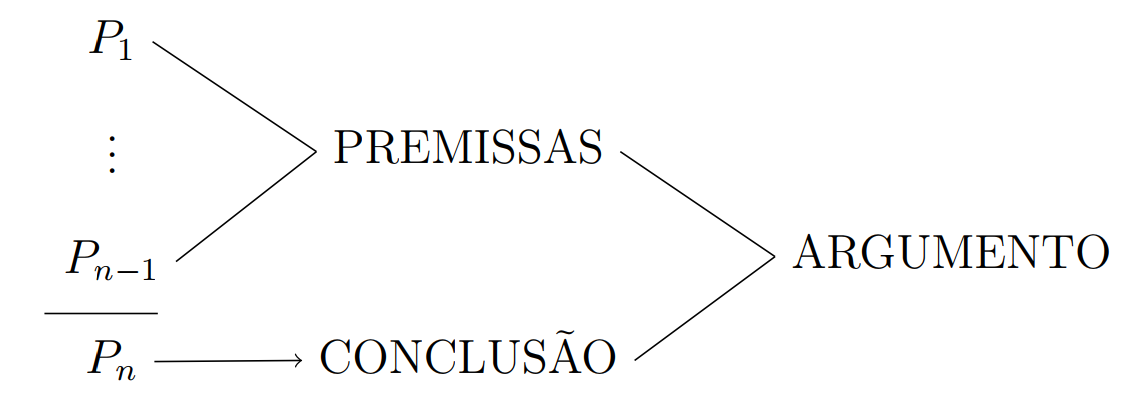
\includegraphics[scale=0.3]{diagramaCapitulo5Grande.png}
	\end{center}
\end{figure}

Diz-se que um argumento é DEDUTIVAMENTE VÁLIDO quando é impossível que a conclusão seja falsa partindo-se de premissas verdadeiras, ou seja, quando a conclusão é consequência lógica das premissas.
Caso contrário, o argumento é dito DEDUTIVAMENTE INVÁLIDO.

Evidentemente será do nosso interesse apenas o estudo dos argumentos dedutivamente válidos.

Vejamos os exemplos:

\begin{align*}
    (ii) & \text{ Se Carla chegar, ganhará a aposta.}\\
         & \text{ Se Carla ganhar a aposta, viajará.}\\
    \text{Logo,}\\
         & \text{ Se Carla chegar, viajará.}
\end{align*}

É importante ressaltar o fato da atenção necessária ao encaminhamento de um raciocínio, a fim de que não se caia em "armadilhas", que nos levam a acreditar que uma forma errada de raciocinar é correta.
Tais formas de argumento ou raciocínio são chamadas de FALÁCIAS.
Por exemplo:

\begin{quote}
    Os estudantes que estudam obtém nota dez. Logo, o melhor que o professor tem a fazer é dar nota dez aos seus alunos.
\end{quote}

% \chapter{ARGUMENTOS NA LÓGICA DE PREDICADOS}

\section{Instanciação Universal (I.U.)}
Seja P(x) uma fórmula e \textit{a} um termo do universo em questão:
\[
\boxed{\frac{\forall x P(x)}{P(a)}}
\]

\noindent \textit{\textbf{Exemplo}}:

TODOS OS HOMENS SÃO PECADORES

TODOS OS PECADORES SERÃO PUNIDOS POR DEUS

SÓCRATES É HOMEM.


\noindent Mostre que o argumento acima é valido.

\section{GENERALIZAÇÃO EXISTENCIAL (G.E.)}
Seja P(x) uma fórmula e \textit{a} um termo do universo em questão:
\[
\boxed{\frac{P(a)}{\exists x P(x)}}
\]

\noindent \textit{\textbf{Exemplo}}:

SÓCRATES É FELIZ E FAMOSO

SE ALGUÉM É FAMOSO OU ELEGANTE, ENTÃO É RENOMADO

PORTANTO, EXISTE ALGUÉM FELIZ E RENOMADO

\noindent Mostre que o argumento acima é válido.

\section{INSTANCIAÇÃO EXISTENCIAL (I.E.)}

\[
\boxed{\frac{\exists x P(x)}{\exists P(a)}}
\]

\begin{itemize}
    \item O termo ``a'' não deve ocorrer nas premissas do argumento. Isto quer dizer que o termo ``a'' só deve aparecer no argumento por força da aplicação da regra I.E.
    \item Uma constante que tenha sido introduzida em um argumento por aplicação da regra I.E. não pode reaparecer, nesse argumento, por uma nova aplicação de I.E.
\end{itemize}

Por exemplo, considere os casos abaixo:
\begin{alignat*}{12}
    \text{a) } & \text{pr}       & \text{1 - } & \exists x P(x) &\\
               & \text{pr}       & \text{2 - } & Q(a) &\\
    \bullet\;  & \text{1, I.E. } & \text{3 - } & P(a) &\\
               & \text{2, 3, C } & \text{4 - } & P(a) \land Q(a) &\\
               & \text{4, G.E. } & \text{5 - } & \exists x (P(x)\ \land Q(x)) &\\
               & & & &\\ % Linha em branco
    \text{b) } & \text{pr}       & \text{1 - } & \exists x Q(x) &\\
               & \text{pr}       & \text{2 - } & \exists x \sim Q(x) &\\
               & \text{1, I.E. } & \text{3 - } & Q(a) &\\
    \bullet\;  & \text{2, I.E. } & \text{4 - } & \sim Q(a) &\\
               & \text{3, 4, C } & \text{5 - } & Q(a)\ \land \sim Q(a) &\\
               & \text{5, G.E. } & \text{6 - } & \exists x (Q(x)\ \land \sim Q(x)) &\\
\end{alignat*}
% \enlargethispage*{\baselineskip}
$\bullet$ INCORRETO
\pagebreak

\noindent \textit{\textbf{Exemplo}}:

ALGUNS ESTUDANTES SÃO DISCIPLINADOS

UM ESTUDANTE DISCIPLINADO RESPEITA SEU MESTRE

LOGO, ALGUNS ESTUDANTES RESPEITAM SEU MESTRE

\noindent Mostre que o argumento acima é valido.

\section{GENERALIZAÇÃO UNIVERSAL (G.U.)}
Seja P(x) uma fórmula e \textit{z} um termo arbitrário do universo em questão:

\[
\boxed{\frac{P(z)}{\forall x P(x)}}
\]

\begin{itemize}
    \item Não se deve aplicar a G.U. a constantes que ocorram nas premissas, pois estas se referem a particulares objetos do domínio.

    \item Não se deve aplicar a G.U a constantes introduzidas pela regra I.E., porque estas também se referem a particulares objetos do domínio.
\end{itemize}

\noindent \textit{\textbf{Exemplo}}:

TODO MUNDO É MARXISTA OU CAPITALISTA

NENHUM ÁRABE É MARXISTA

LOGO, TODOS OS ÁRABES SÃO CAPITALISTAS

\noindent Mostre que o argumento acima é válido.

\bigskip
\noindent \textbf{EXERCÍCIOS:}
\begin{enumerate}[label=\arabic*)]
    \item Use as regras de inferência para mostrar a validade dos argumentos abaixo:
    \begin{enumerate}[label=\alph*)]
        \item Todos os membros da Associação vivem na cidade. Quem é presidente  da sociedade é membro da Associação. Sra. Farias é presidente da Sociedade. Logo, Sra. Farias vive na cidade.
        \item Todas as linguagens de programação são importantes. Nenhuma linguagem de programação importante será dispensada. PROLOG é uma linguagem de programação. Logo, há linguagens de programação que não são dispensadas.
        \item Todas as vítimas são inocentes. Todos os inocentes serão absolvidos pela justiça. Maria é vítima, logo Maria será absolvida pela justiça.
        \item Paulo é estudioso e simpático. Se alguém é simpático ou inteligente, então é popular. Portanto, existe alguém estudioso e popular.
        \item Alguns soldados são heróis. Portanto, os heróis são valentes. Logo, alguns soldados são valentes.
    \end{enumerate}
\end{enumerate}


\end{document}
